%%%%%%%%%%%%%%%%%%%%%%%%%%%%%%%%%%%%%%%%%%%%%%%%%%%%%%%%%%%%%%%%%%%%%%
% Template for a UBC-compliant dissertation
% At the minimum, you will need to change the information found
% after the "Document meta-data"
%
%!TEX TS-program = pdflatex
%!TEX encoding = UTF-8 Unicode

%% The ubcdiss class provides several options:
%%   gpscopy (aka fogscopy)
%%       set parameters to exactly how GPS specifies
%%         * single-sided
%%         * page-numbering starts from title page
%%         * the lists of figures and tables have each entry prefixed
%%           with 'Figure' or 'Table'
%%       This can be tested by `\ifgpscopy ... \else ... \fi'
%%   10pt, 11pt, 12pt
%%       set default font size
%%   oneside, twoside
%%       whether to format for single-sided or double-sided printing
%%   balanced
%%       when double-sided, ensure page content is centred
%%       rather than slightly offset (the default)
%%   singlespacing, onehalfspacing, doublespacing
%%       set default inter-line text spacing; the ubcdiss class
%%       provides \textspacing to revert to this configured spacing
%%   draft
%%       disable more intensive processing, such as including
%%       graphics, etc.
%%

% For submission to GPS
\documentclass[gpscopy,onehalfspacing,11pt]{ubcdiss}

% For your own copies (looks nicer)
% \documentclass[balanced,twoside,11pt]{ubcdiss}

%%%%%%%%%%%%%%%%%%%%%%%%%%%%%%%%%%%%%%%%%%%%%%%%%%%%%%%%%%%%%%%%%%%%%%
%%%%%%%%%%%%%%%%%%%%%%%%%%%%%%%%%%%%%%%%%%%%%%%%%%%%%%%%%%%%%%%%%%%%%%
%%
%% FONTS:
%%
%% The defaults below configures Times Roman for the serif font,
%% Helvetica for the sans serif font, and Courier for the
%% typewriter-style font.  Configuring fonts can be time
%% consuming; we recommend skipping to END FONTS!
%%
%% If you're feeling brave, have lots of time, and wish to use one
%% your platform's native fonts, see the commented out bits below for
%% XeTeX/XeLaTeX.  This is not for the faint at heart.
%% (And shouldn't you be writing? :-)
%%

%% NFSS font specification (New Font Selection Scheme)
\usepackage{times,mathptmx,courier}
\usepackage[scaled=.92]{helvet}
\usepackage{float}
\usepackage[]{algorithm2e}
\usepackage{ifthen}
\usepackage[normalem]{ulem} % for \sout
\usepackage{xcolor}
\usepackage{amssymb}
%% Math or theory people may want to include the handy AMS macros
%\usepackage{amssymb}
\usepackage{amsmath}
%\usepackage{amsfonts}
% to force the figures to appear where i want!!
\usepackage{float}
%% The pifont package provides access to the elements in the dingbat font.
%% Use \ding{##} for a particular dingbat (see p7 of psnfss2e.pdf)
%%   Useful:
%%     51,52 different forms of a checkmark
%%     54,55,56 different forms of a cross (saltyre)
%%     172-181 are 1-10 in open circle (serif)
%%     182-191 are 1-10 black circle (serif)
%%     192-201 are 1-10 in open circle (sans serif)
%%     202-211 are 1-10 in black circle (sans serif)
%% \begin{dinglist}{##}\item... or dingautolist (which auto-increments)
%% to create a bullet list with the provided character.
\usepackage{pifont}

%%%%%%%%%%%%%%%%%%%%%%%%%%%%%%%%%%%%%%%%%%%%%%%%%%%%%%%%%%%%%%%%%%%%%%
%% Configure fonts for XeTeX / XeLaTeX using the fontspec package.
%% Be sure to check out the fontspec documentation.
%\usepackage{fontspec,xltxtra,xunicode}	% required
%\defaultfontfeatures{Mapping=tex-text}	% recommended
%% Minion Pro and Myriad Pro are shipped with some versions of
%% Adobe Reader.  Adobe representatives have commented that these
%% fonts can be used outside of Adobe Reader.
%\setromanfont[Numbers=OldStyle]{Minion Pro}
%\setsansfont[Numbers=OldStyle,Scale=MatchLowercase]{Myriad Pro}
%\setmonofont[Scale=MatchLowercase]{Andale Mono}

%% Other alternatives:
%\setromanfont[Mapping=tex-text]{Adobe Caslon}
%\setsansfont[Scale=MatchLowercase]{Gill Sans}
%\setsansfont[Scale=MatchLowercase,Mapping=tex-text]{Futura}
%\setmonofont[Scale=MatchLowercase]{Andale Mono}
%\newfontfamily{\SYM}[Scale=0.9]{Zapf Dingbats}
%% END FONTS
%%%%%%%%%%%%%%%%%%%%%%%%%%%%%%%%%%%%%%%%%%%%%%%%%%%%%%%%%%%%%%%%%%%%%%
%%%%%%%%%%%%%%%%%%%%%%%%%%%%%%%%%%%%%%%%%%%%%%%%%%%%%%%%%%%%%%%%%%%%%%



%%%%%%%%%%%%%%%%%%%%%%%%%%%%%%%%%%%%%%%%%%%%%%%%%%%%%%%%%%%%%%%%%%%%%%
%%%%%%%%%%%%%%%%%%%%%%%%%%%%%%%%%%%%%%%%%%%%%%%%%%%%%%%%%%%%%%%%%%%%%%
%%
%% Recommended packages
%%
\usepackage{checkend}	% better error messages on left-open environments
\usepackage{graphicx}	% for incorporating external images

%% booktabs: provides some special commands for typesetting tables as used
%% in excellent journals.  Ignore the examples in the Lamport book!
\usepackage{booktabs}

%% listings: useful support for including source code listings, with
%% optional special keyword formatting.  The \lstset{} causes
%% the text to be typeset in a smaller sans serif font, with
%% proportional spacing.
\usepackage{listings}
\lstset{basicstyle=\sffamily\scriptsize,showstringspaces=false,fontadjust}

%% The acronym package provides support for defining acronyms, providing
%% their expansion when first used, and building glossaries.  See the
%% example in glossary.tex and the example usage throughout the example
%% document.
%% NOTE: to use \MakeTextLowercase in the \acsfont command below,
%%   we *must* use the `nohyperlinks' option -- it causes errors with
%%   hyperref otherwise.  See Section 5.2 in the ``LaTeX 2e for Class
%%   and Package Writers Guide'' (clsguide.pdf) for details.
\usepackage[printonlyused,nohyperlinks]{acronym}
%% The ubcdiss.cls loads the `textcase' package which provides commands
%% for upper-casing and lower-casing text.  The following causes
%% the acronym package to typeset acronyms in small-caps
%% as recommended by Bringhurst.
\renewcommand{\acsfont}[1]{{\scshape \MakeTextLowercase{#1}}}

%% color: add support for expressing colour models.  Grey can be used
%% to great effect to emphasize other parts of a graphic or text.
%% For an excellent set of examples, see Tufte's "Visual Display of
%% Quantitative Information" or "Envisioning Information".
\usepackage{color}
\definecolor{greytext}{gray}{0.5}

%% comment: provides a new {comment} environment: all text inside the
%% environment is ignored.
%%   \begin{comment} ignored text ... \end{comment}
\usepackage{comment}

%% The natbib package provides more sophisticated citing commands
%% such as \citeauthor{} to provide the author names of a work,
%% \citet{} to produce an author-and-reference citation,
%% \citep{} to produce a parenthetical citation.
%% We use \citeeg{} to provide examples
\usepackage[numbers,sort&compress]{natbib}
\newcommand{\citeeg}[1]{\citep[e.g.,][]{#1}}

%% The titlesec package provides commands to vary how chapter and
%% section titles are typeset.  The following uses more compact
%% spacings above and below the title.  The titleformat that follow
%% ensure chapter/section titles are set in singlespace.
\usepackage[compact]{titlesec}
\titleformat*{\section}{\singlespacing\raggedright\bfseries\Large}
\titleformat*{\subsection}{\singlespacing\raggedright\bfseries\large}
\titleformat*{\subsubsection}{\singlespacing\raggedright\bfseries}
\titleformat*{\paragraph}{\singlespacing\raggedright\itshape}

%% The caption package provides support for varying how table and
%% figure captions are typeset.
\usepackage[format=hang,indention=-1cm,labelfont={bf},margin=1em]{caption}

%% url: for typesetting URLs and smart(er) hyphenation.
%% \url{http://...}
\usepackage{url}
\urlstyle{sf}	% typeset urls in sans-serif


%%%%%%%%%%%%%%%%%%%%%%%%%%%%%%%%%%%%%%%%%%%%%%%%%%%%%%%%%%%%%%%%%%%%%%
%%%%%%%%%%%%%%%%%%%%%%%%%%%%%%%%%%%%%%%%%%%%%%%%%%%%%%%%%%%%%%%%%%%%%%
%%
%% Possibly useful packages: you may need to explicitly install
%% these from CTAN if they aren't part of your distribution;
%% teTeX seems to ship with a smaller base than MikTeX and MacTeX.
%%
%\usepackage{pdfpages}	% insert pages from other PDF files
%\usepackage{longtable}	% provide tables spanning multiple pages
%\usepackage{chngpage}	% support changing the page widths on demand
%\usepackage{tabularx}	% an enhanced tabular environment

%% enumitem: support pausing and resuming enumerate environments.
\usepackage{enumitem}

%% rotating: provides two environments, sidewaystable and sidewaysfigure,
%% for typesetting tables and figures in landscape mode.
%\usepackage{rotating}

%% subfig: provides for including subfigures within a figure,
%% and includes being able to separately reference the subfigures.
%\usepackage{subfig}

%% ragged2e: provides several new new commands \Centering, \RaggedLeft,
%% \RaggedRight and \justifying and new environments Center, FlushLeft,
%% FlushRight and justify, which set ragged text and are easily
%% configurable to allow hyphenation.
%\usepackage{ragged2e}

%% The ulem package provides a \sout{} for striking out text and
%% \xout for crossing out text.  The normalem and normalbf are
%% necessary as the package messes with the emphasis and bold fonts
%% otherwise.
%\usepackage[normalem,normalbf]{ulem}    % for \sout

%%%%%%%%%%%%%%%%%%%%%%%%%%%%%%%%%%%%%%%%%%%%%%%%%%%%%%%%%%%%%%%%%%%%%%
%% HYPERREF:
%% The hyperref package provides for embedding hyperlinks into your
%% document.  By default the table of contents, references, citations,
%% and footnotes are hyperlinked.
%%
%% Hyperref provides a very handy command for doing cross-references:
%% \autoref{}.  This is similar to \ref{} and \pageref{} except that
%% it automagically puts in the *type* of reference.  For example,
%% referencing a figure's label will put the text `Figure 3.4'.
%% And the text will be hyperlinked to the appropriate place in the
%% document.
%%
%% Generally hyperref should appear after most other packages

%% The following puts hyperlinks in very faint grey boxes.
%% The `pagebackref' causes the references in the bibliography to have
%% back-references to the citing page; `backref' puts the citing section
%% number.  See further below for other examples of using hyperref.
%% 2009/12/09: now use `linktocpage' (Jacek Kisynski): GPS now prefers
%%   that the ToC, LoF, LoT place the hyperlink on the page number,
%%   rather than the entry text.
\usepackage[bookmarks,bookmarksnumbered,%
    allbordercolors={0.8 0.8 0.8},%
    pagebackref,linktocpage%
    ]{hyperref}
%% The following change how the the back-references text is typeset in a
%% bibliography when `backref' or `pagebackref' are used
%%
%% Change \nocitations if you'd like some text shown where there
%% are no citations found (e.g., pulled in with \nocite{xxx})
\newcommand{\nocitations}{\relax}
%%\newcommand{\nocitations}{No citations}
%%
%\renewcommand*{\backref}[1]{}% necessary for backref < 1.33
\renewcommand*{\backrefsep}{,~}%
\renewcommand*{\backreftwosep}{,~}% ', and~'
\renewcommand*{\backreflastsep}{,~}% ' and~'
\renewcommand*{\backrefalt}[4]{%
\textcolor{greytext}{\ifcase #1%
\nocitations%
\or
\(\rightarrow\) page #2%
\else
\(\rightarrow\) pages #2%
\fi}}


%% The following uses most defaults, which causes hyperlinks to be
%% surrounded by colourful boxes; the colours are only visible in
%% PDFs and don't show up when printed:
%\usepackage[bookmarks,bookmarksnumbered]{hyperref}

%% The following disables the colourful boxes around hyperlinks.
%\usepackage[bookmarks,bookmarksnumbered,pdfborder={0 0 0}]{hyperref}

%% The following disables all hyperlinking, but still enabled use of
%% \autoref{}
%\usepackage[draft]{hyperref}

%% The following commands causes chapter and section references to
%% uppercase the part name.
\renewcommand{\chapterautorefname}{Chapter}
\renewcommand{\sectionautorefname}{Section}
\renewcommand{\subsectionautorefname}{Section}
\renewcommand{\subsubsectionautorefname}{Section}

%% If you have long page numbers (e.g., roman numbers in the
%% preliminary pages for page 28 = xxviii), you might need to
%% uncomment the following and tweak the \@pnumwidth length
%% (default: 1.55em).  See the tocloft documentation at
%% http://www.ctan.org/tex-archive/macros/latex/contrib/tocloft/
% \makeatletter
% \renewcommand{\@pnumwidth}{3em}
% \makeatother

%%%%%%%%%%%%%%%%%%%%%%%%%%%%%%%%%%%%%%%%%%%%%%%%%%%%%%%%%%%%%%%%%%%%%%
%%%%%%%%%%%%%%%%%%%%%%%%%%%%%%%%%%%%%%%%%%%%%%%%%%%%%%%%%%%%%%%%%%%%%%
%%
%% Some special settings that controls how text is typeset
%%
% \raggedbottom		% pages don't have to line up nicely on the last line
% \sloppy		% be a bit more relaxed in inter-word spacing
% \clubpenalty=10000	% try harder to avoid orphans
% \widowpenalty=10000	% try harder to avoid widows
% \tolerance=1000

%% And include some of our own useful macros
% This file provides examples of some useful macros for typesetting
% dissertations.  None of the macros defined here are necessary beyond
% for the template documentation, so feel free to change, remove, and add
% your own definitions.
%
% We recommend that you define macros to separate the semantics
% of the things you write from how they are presented.  For example,
% you'll see definitions below for a macro \file{}: by using
% \file{} consistently in the text, we can change how filenames
% are typeset simply by changing the definition of \file{} in
% this file.
% 
%% The following is a directive for TeXShop to indicate the main file
%%!TEX root = diss.tex

\newcommand{\NA}{\textsc{n/a}}	% for "not applicable"
\newcommand{\eg}{e.g.,\ }	% proper form of examples (\eg a, b, c)
\newcommand{\ie}{i.e.,\ }	% proper form for that is (\ie a, b, c)
\newcommand{\etal}{\emph{et al}}

% Some useful macros for typesetting terms.
\newcommand{\file}[1]{\texttt{#1}}
\newcommand{\class}[1]{\texttt{#1}}
\newcommand{\latexpackage}[1]{\href{http://www.ctan.org/macros/latex/contrib/#1}{\texttt{#1}}}
\newcommand{\latexmiscpackage}[1]{\href{http://www.ctan.org/macros/latex/contrib/misc/#1.sty}{\texttt{#1}}}
\newcommand{\env}[1]{\texttt{#1}}
\newcommand{\BibTeX}{Bib\TeX}

% Define a command \doi{} to typeset a digital object identifier (DOI).
% Note: if the following definition raise an error, then you likely
% have an ancient version of url.sty.  Either find a more recent version
% (3.1 or later work fine) and simply copy it into this directory,  or
% comment out the following two lines and uncomment the third.
\DeclareUrlCommand\DOI{}
\newcommand{\doi}[1]{\href{http://dx.doi.org/#1}{\DOI{doi:#1}}}
%\newcommand{\doi}[1]{\href{http://dx.doi.org/#1}{doi:#1}}

% Useful macro to reference an online document with a hyperlink
% as well with the URL explicitly listed in a footnote
% #1: the URL
% #2: the anchoring text
\newcommand{\webref}[2]{\href{#1}{#2}\footnote{\url{#1}}}

% epigraph is a nice environment for typesetting quotations
\makeatletter
\newenvironment{epigraph}{%
	\begin{flushright}
	\begin{minipage}{\columnwidth-0.75in}
	\begin{flushright}
	\@ifundefined{singlespacing}{}{\singlespacing}%
    }{
	\end{flushright}
	\end{minipage}
	\end{flushright}}
\makeatother

% \FIXME{} is a useful macro for noting things needing to be changed.
% The following definition will also output a warning to the console
\newcommand{\FIXME}[1]{\typeout{**FIXME** #1}\textbf{[FIXME: #1]}}


\newcommand{\dinv}{Dinv}
%%
%%\newcommand{\cone}{What state should be logged?\xspace}
%%
%%\newcommand{\ctwo}{At what point should state be logged?\xspace}
%%
%%\newcommand{\cthree}{What state should be tested for invariants?\xspace}
%%
%%\newcommand{\cfour}{When do distributed invariants hold?\xspace}
%%
%%\newcommand{\cfive}{How can distributed state be prepared for analysis with
%%Daikon?\xspace}

\newcommand{\cone}{What state should be logged and when?}
\newcommand{\ctwo}{How to infer distributed invariants from logged state?}
\newcommand{\cthree}{How to enforce inferred distributed invariants?}
%%
\newcommand{\csix}{How can inferred invariants be checked in future
executions?\xspace} \newcommand{\scc}{strongly consistent cut}
% END





%%%%%%%%%%%%%%%%%%%%%%%%%%%%%%%%%%%%%%%%%%%%%%%%%%%%%%%%%%%%%%%%%%%%%%
%%%%%%%%%%%%%%%%%%%%%%%%%%%%%%%%%%%%%%%%%%%%%%%%%%%%%%%%%%%%%%%%%%%%%%
%%
%% Document meta-data: be sure to also change the \hypersetup information
%%

\title{The unbalancing act: proxy preservation for censorship resistance systems}

\author{Jodi Spacek}
\previousdegree{Bachelor of Computer Science, UBC, 2014}
\previousdegree{Bachelor of Music, Mount Allison University, 2000}

% What is this dissertation for?
\degreetitle{Master of Science}

\institution{The University of British Columbia}
\campus{Vancouver}

\faculty{The Faculty of Graduate and Postdoctoral Studies}
\department{Computer Science}
\submissionmonth{April}
\submissionyear{2019}

% details of your examining committee
\examiningcommittee{Ivan Beschastnikh, Computer Science}{Supervisor}
\examiningcommittee{Norman Hutchinson, Computer Science}%
    {Supervisory Committee Member}

% details of your supervisory committee
% \supervisorycommittee{Ira Crater, Materials Engineering}%
%     {Supervisory Committee Member}
% \supervisorycommittee{Adeline Long, \textsc{CEO} of Aerial Machine
%     Transportation, Inc.}{Supervisory Committee Member}

%% hyperref package provides support for embedding meta-data in .PDF
%% files
\hypersetup{
  pdftitle={PDF Title (DRAFT: \today)},
  pdfauthor={PDF Author},
  pdfkeywords={Keyword 1, Keyword 2}
}

%%%%%%%%%%%%%%%%%%%%%%%%%%%%%%%%%%%%%%%%%%%%%%%%%%%%%%%%%%%%%%%%%%%%%%
%%%%%%%%%%%%%%%%%%%%%%%%%%%%%%%%%%%%%%%%%%%%%%%%%%%%%%%%%%%%%%%%%%%%%%
%%
%% The document content
%%

%% LaTeX's \includeonly commands causes any uses of \include{} to only
%% include files that are in the list.  This is helpful to produce
%% subsets of your thesis (e.g., for committee members who want to see
%% the dissertation chapter by chapter).  It also saves time by
%% avoiding reprocessing the entire file.
%\includeonly{intro,conclusions}
%\includeonly{discussion}

\begin{document}

%%%%%%%%%%%%%%%%%%%%%%%%%%%%%%%%%%%%%%%%%%%%%%%%%%
%% From Thesis Components: Tradtional Thesis
%% <http://www.grad.ubc.ca/current-students/dissertation-thesis-preparation/order-components>

% Preliminary Pages (numbered in lower case Roman numerals)
%    1. Title page (mandatory)
\maketitle

%    2. Committee page (mandatory): lists supervisory committee and,
%    if applicable, the examining committee
\makecommitteepage

%    3. Abstract (mandatory - maximum 350 words)
\chapter{Abstract}
\label{sec:abstract}

Internet censorship is a form of digital authoritarianism in certain countries that restrict access to the internet. Internet freedom, to a degree, is possible even in these countries by means of proxies maintained outside of the censor's boundaries. These proxies can be compromised by censors who pose as legitimate users to discover proxies. Censors are powerful adversaries and may block access to any proxy once they know about it.

We propose a novel technique to address the proxy distribution problem in this thesis. We introduce the \textit{needle} algorithm that preserves proxies by limiting their distribution. The number of proxies preserved is controlled by the algorithm's parameters. We show that it is a useful mechanism for preserving proxies under a censorship threat model. 

We examine characteristics of the algorithm in a simulation. Three measures are important under the censorship threat model; the enumeration or discovery of all proxies, load balancing, and the collateral damage of innocent bystanders. We compare the results of these experiments with two well-known algorithms, uniform random and power of 2 choices, as well as Tor's \texttt{bridgedb} proxy assignment mechanism. 
\cleardoublepage

%    4. Lay Summary (Effective May 2017, mandatory - maximum 150 words)
%% The following is a directive for TeXShop to indicate the main file
%%!TEX root = diss.tex

%% https://www.grad.ubc.ca/current-students/dissertation-thesis-preparation/preliminary-pages
%% 
%% LAY SUMMARY Effective May 2017, all theses and dissertations must
%% include a lay summary.  The lay or public summary explains the key
%% goals and contributions of the research/scholarly work in terms that
%% can be understood by the general public. It must not exceed 150
%% words in length.

\chapter{Lay Summary}
Internet censorship prevents citizens of a country from accessing content on specific websites. Censors are powerful figures that restrict free access to information by limiting their citizens' internet access when they are within the censor's country. A proxy is a single hop beyond the reach of the censor that is controlled by an organization on the outside. A censored user connects to the proxy to hop outside of their country to view restricted content. There are not enough proxies for each censored user to have their own, so they must share. A censor may pretend to be honest to learn about the proxies to block access to them. This thesis presents an approach to proxy distribution that preserves some proxies by restricting their distribution. We examine the lifetime of proxies in a simulation to see if this solution is practical in a real-life setting. 
\cleardoublepage

%    5. Preface
%% The following is a directive for TeXShop to indicate the main file
%%!TEX root = diss.tex

\chapter{Preface} 

The original and unpublished work presented in this thesis was conducted by the author in the \ac{NSS} lab in the Department of Computer Science at the \ac{UBC} in Vancouver. It was designed, documented, and written with assistance from Dr. Ivan Beschastnikh, Dr. Norman Hutchinson, and Dr. William Aiello. Figures \ref{fig:simplecensor}, \ref{fig:censorblock}, and \ref{fig:proxydistro} were created by Carlo Cossette. All other figures, tables, and experiments were designed and conducted by the author.

\cleardoublepage

%    6. Table of contents (mandatory - list all items in the preliminary pages
%    starting with the abstract, followed by chapter headings and
%    subheadings, bibliographies and appendices)
\tableofcontents
\cleardoublepage	% required by tocloft package

%    7. List of tables (mandatory if thesis has tables)
\listoftables
\cleardoublepage	% required by tocloft package

%    8. List of figures (mandatory if thesis has figures)
\listoffigures
\cleardoublepage	% required by tocloft package

%    9. List of illustrations (mandatory if thesis has illustrations)
%   10. Lists of symbols, abbreviations or other (optional)

%   11. Glossary (optional)
%% The following is a directive for TeXShop to indicate the main file
%%!TEX root = diss.tex

\chapter{Glossary}

% This glossary uses the handy \latexpackage{acroynym} package to automatically
% maintain the glossary.  It uses the package's \texttt{printonlyused}
% option to include only those acronyms explicitly referenced in the
% \LaTeX\ source.

% use \acrodef to define an acronym, but no listing
\acrodef{UI}{user interface}

% The acronym environment will typeset only those acronyms that were
% *actually used* in the course of the document
\begin{acronym}[ANOVA]
\acrodef{NSERC}{Natural Science and Engineering Research Council of Canada}
\acrodef{NSS}{Networks, Systems, and Security}
\acrodef{UBC}{University of British Columbia}

\acro{ANOVA}[ANOVA]{Analysis of Variance\acroextra{, a set of
  statistical techniques to identify sources of variability between groups}}
\acro{CTAN}{\acroextra{The }Common \TeX\ Archive Network}
\acro{DOI}{Document Object Identifier\acroextra{ (see
    \url{http://doi.org})}}
\acro{GPS}[GPS]{Graduate and Postdoctoral Studies}
\acro{PDF}{Portable Document Format}
\acro{RCS}[RCS]{Revision control system\acroextra{, a software
    tool for tracking changes to a set of files}}
\acro{TLX}[TLX]{Task Load Index\acroextra{, an instrument for gauging
  the subjective mental workload experienced by a human in performing
  a task}}
\acro{UML}{Unified Modelling Language\acroextra{, a visual language
    for modelling the structure of software artefacts}}
\acro{URL}{Unique Resource Locator\acroextra{, used to describe a
    means for obtaining some resource on the world wide web}}
\acro{W3C}[W3C]{\acroextra{the }World Wide Web Consortium\acroextra{,
    the standards body for web technologies}}
\acro{XML}{Extensible Markup Language}
%%%%%
\acrodef{CGS-M}{Canada Graduate Scholarships-Master's}

\acro{CCP}{Coupon Collector Problem}
\acro{CCP-R}{Coupon Collector Problem Ring}
\acro{CDN}{Content Delivery Networks}
\acro{CRS}{Censorship Resistance Systems}

\acro{DNS}{Domain Name System}

\acro{HTTP}{Hypertext Transfer Protocol}
\acro{HTTPS}{Hypertext Transfer Protocol Secure}

\acro{IP}{Internet Protocol}
\acro{ISP}{Internet Service Providers}

\acro{OONI}{Open Observatory of Network Interference}


\end{acronym}

% You can also use \newacro{}{} to only define acronyms
% but without explictly creating a glossary
% 
% \newacro{ANOVA}[ANOVA]{Analysis of Variance\acroextra{, a set of
%   statistical techniques to identify sources of variability between groups.}}
% \newacro{API}[API]{application programming interface}
% \newacro{GOMS}[GOMS]{Goals, Operators, Methods, and Selection\acroextra{,
%   a framework for usability analysis.}}
% \newacro{TLX}[TLX]{Task Load Index\acroextra{, an instrument for gauging
%   the subjective mental workload experienced by a human in performing
%   a task.}}
% \newacro{UI}[UI]{user interface}
% \newacro{UML}[UML]{Unified Modelling Language}
% \newacro{W3C}[W3C]{World Wide Web Consortium}
% \newacro{XML}[XML]{Extensible Markup Language}	% always input, since other macros may rely on it

\textspacing		% begin one-half or double spacing

%   12. Acknowledgements (optional)
%% The following is a directive for TeXShop to indicate the main file
%%!TEX root = diss.tex

\chapter{Acknowledgements}

This research was funded by a Canada Graduate Scholarships-Master’s (CGS-M) grant from the Natural Science and Engineering Research Council of Canada (NSERC).

%   13. Dedication (optional)

% Body of Thesis (not all sections may apply)
\mainmatter

\acresetall	% reset all acronyms used so far

\newcommand{\ra}{$\rightarrow$}
\newboolean{showedits}
\setboolean{showedits}{true} % toggle to show or hide edits
\ifthenelse{\boolean{showedits}}
{
	\newcommand{\ugh}[1]{\textcolor{red}{\uwave{#1}}} % please rephrase
	\newcommand{\ins}[1]{\textcolor{blue}{\uline{#1}}} % please insert
	\newcommand{\del}[1]{\textcolor{red}{\sout{#1}}} % please delete
	\newcommand{\chg}[2]{\textcolor{red}{\sout{#1}}{\ra}\textcolor{blue}{\uline{#2}}} % please change
}{
	\newcommand{\ugh}[1]{#1} % please rephrase
	\newcommand{\ins}[1]{#1} % please insert
	\newcommand{\del}[1]{} % please delete
	\newcommand{\chg}[2]{#2}
}

\newboolean{showcomments}
%\setboolean{showcomments}{true}
\setboolean{showcomments}{true}
\newcommand{\id}[1]{$-$Id: scgPaper.tex 32478 2010-04-29 09:11:32Z oscar $-$}
\newcommand{\yellowbox}[1]{\fcolorbox{gray}{yellow}{\bfseries\sffamily\scriptsize#1}}
\newcommand{\triangles}[1]{{\sf\small$\blacktriangleright$\textit{#1}$\blacktriangleleft$}}
\ifthenelse{\boolean{showcomments}}
%{\newcommand{\nb}[2]{{\yellowbox{#1}\triangles{#2}}}
{\newcommand{\nbc}[3]{
 {\colorbox{#3}{\bfseries\sffamily\scriptsize\textcolor{white}{#1}}}
 {\textcolor{#3}{\sf\small$\blacktriangleright$\textit{#2}$\blacktriangleleft$}}}
 \newcommand{\version}{\emph{\scriptsize\id}}}
{\newcommand{\nbc}[3]{}
 \renewcommand{\ugh}[1]{#1} % please rephrase
 \renewcommand{\ins}[1]{#1} % please insert
 \renewcommand{\del}[1]{} % please delete
 \renewcommand{\chg}[2]{#2} % please change
 \newcommand{\version}{}}
\newcommand{\nb}[2]{\nbc{#1}{#2}{orange}}

\definecolor{ibcolor}{rgb}{0.9,0.5,0}
\definecolor{jscolor}{rgb}{1,0,1}

%% \definecolor{bocolor}{rgb}{0.6,0.9,0.2}
%% \definecolor{jrcolor}{rgb}{0.5,0,0.5}
%% \definecolor{hkcolor}{rgb}{0.4,0.1,0}
%% \definecolor{nrcolor}{rgb}{1.0,0.6,0.1}
\definecolor{tdcolor}{rgb}{1.0,0,0}

\newcommand\ivan[1]{\nbc{IB}{#1}{ibcolor}}
\newcommand\jodi[1]{\nbc{JS}{#1}{jscolor}}
\newcommand\todo[1]{\nbc{TODO}{#1}{tdcolor}}

%%\newcommand{\ars}[1]{\textcolor{magenta}{[[#1]]}} 
%% \newcommand\dm[1]{\nbc{DM}{#1}{dmcolor}}
%% \newcommand\tg[1]{\nbc{TG}{#1}{tgcolor}}
%% \newcommand\kb[1]{\nbc{KB}{#1}{kbcolor}}

%\usepackage{wasysym}[nointegrals]

\newcommand\yesml[1]{\nbc{ML {\textcolor{yellow}\sun}}{#1}{mircolor}}

\chapter{Introduction}
\label{sec:intro} 

%%%%%%%%%%%%%%%%%%%%%%%%%%%%%%%%%%%%%%%%%%%%%%%%%%%%%%%%%%%%%%%%%%%%%%
\begin{figure*}[h!]
\centering
     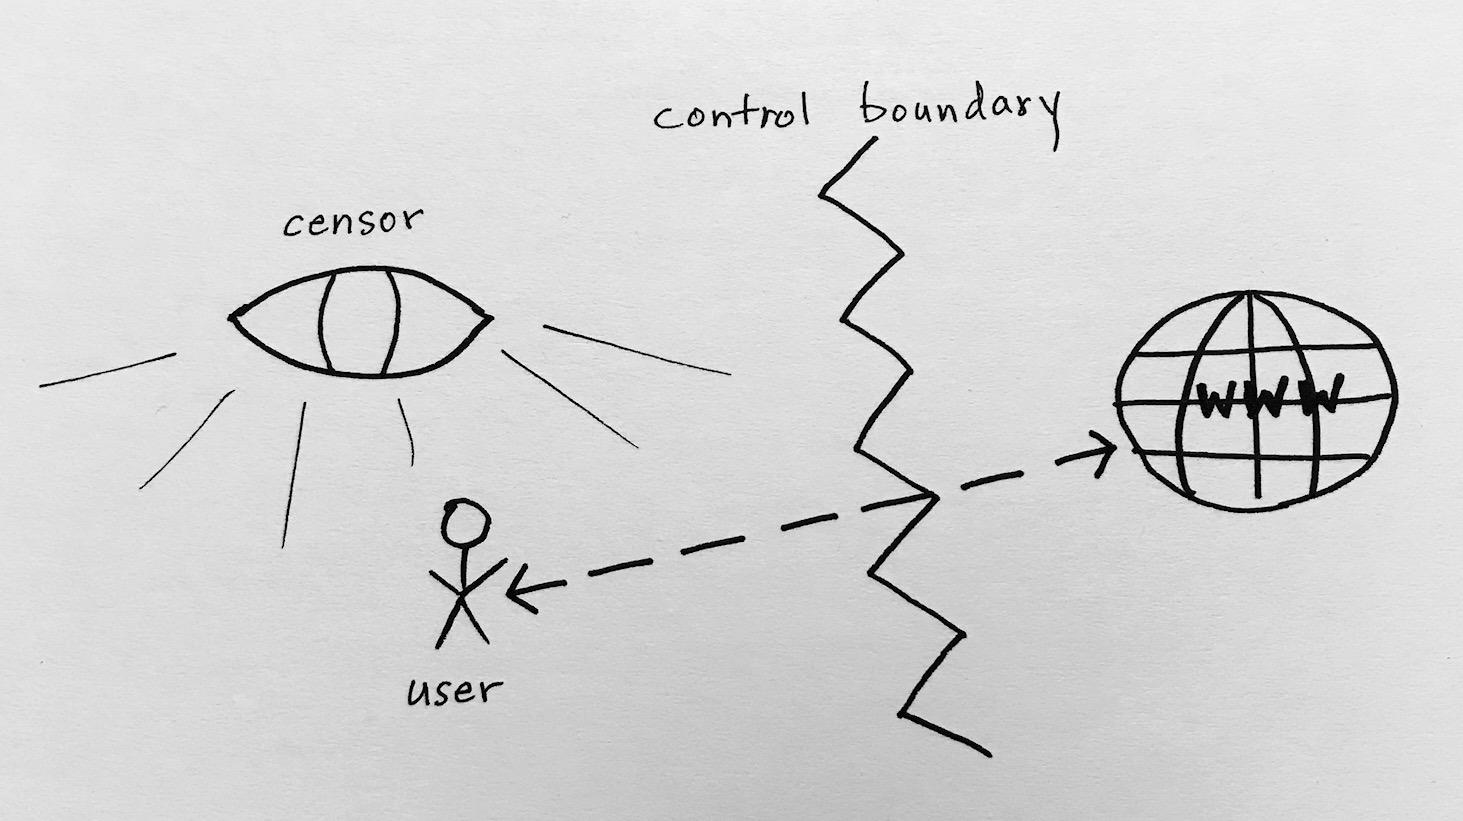
\includegraphics[width=1.0\textwidth]{fig/censor_simple.png}
    \caption{A censor observes a citizen's network activity to the internet outside its control boundary.}
    
    \label{fig:simplecensor}
\end{figure*}
%%%%%%%%%%%%%%%%%%%%%%%%%%%%%%%%%%%%%%%%%%%%%%%%%%%%%%%%%%%%%%%%%%%%%%

Internet censorship is a significant and growing problem that threatens our freedom of expression and access to information. A citizen within a censored country attempts to access the internet that is hosted beyond the censor's control boundary, shown in Figure \ref{fig:simplecensor}. A censor is a strong nation state adversary that conducts mass surveillance and utilizes blacklists. One of the simplest techniques employed by censors is to deny access to users by blocking traffic destined for blacklisted sites. 

%%%%%%%%%%%%%%%%%%%%%%%%%%%%%%%%%%%%%%%%%%%%%%%%%%%%%%%%%%%%%%%%%%%%%%
\begin{figure*}[h!]
\centering
     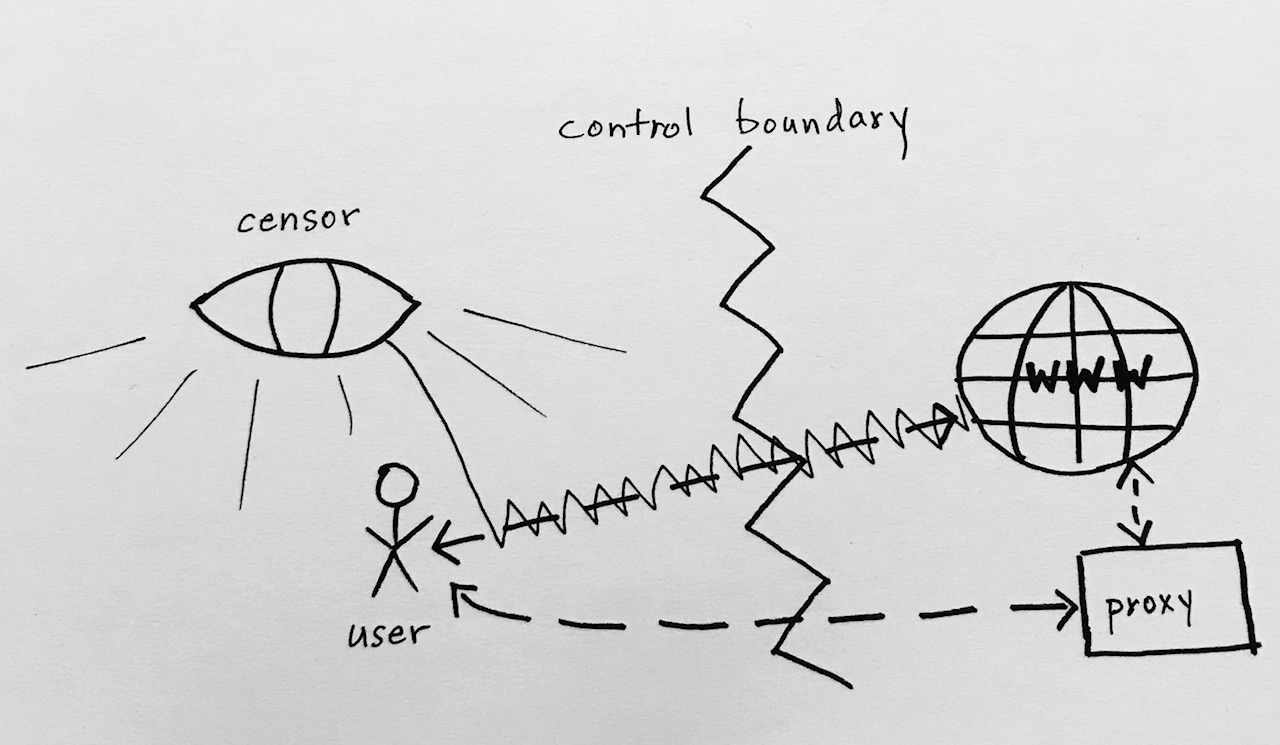
\includegraphics[width=1.0\textwidth]{fig/censor_block.png}
    \caption{A censor blocks direct access to a site but the citizen uses a proxy to access the internet.}
    
    \label{fig:censorblock}
\end{figure*}
%%%%%%%%%%%%%%%%%%%%%%%%%%%%%%%%%%%%%%%%%%%%%%%%%%%%%%%%%%%%%%%%%%%%%%

This effective censorship technique is circumvented by means of proxies; single-hop servers outside of the censored country that facilitate indirect access to censored information. In Figure \ref{fig:censorblock}, a citizen is blocked from the internet but manages to access sites via a proxy. Censorship resistance systems manage proxies and allow users in censored countries to access blacklisted websites. These systems bypass censors and route users through secret paths. Secret paths rely on proxies that are managed by censorship resistance systems. Proxies serve as intermediary hops between a user and a blacklisted destination site.

%%%%%%%%%%%%%%%%%%%%%%%%%%%%%%%%%%%%%%%%%%%%%%%%%%%%%%%%%%%%%%%%%%%%%%
\begin{figure*}[h!]
\centering
     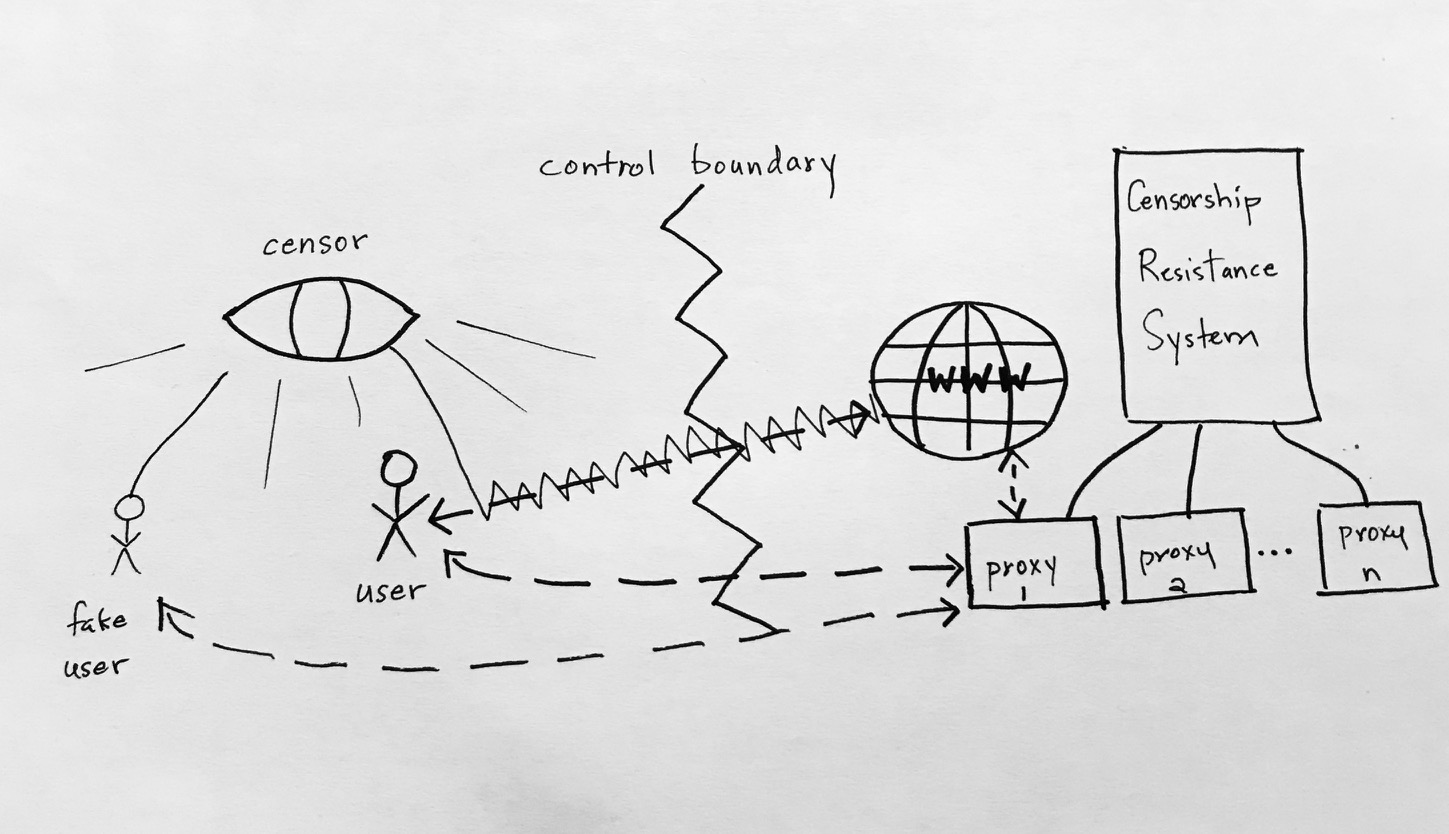
\includegraphics[width=1.0\textwidth]{fig/censor_crs.png}
    \caption{Censorship circumvention via proxy distribution.}
    \label{fig:proxydistro}
\end{figure*}
%%%%%%%%%%%%%%%%%%%%%%%%%%%%%%%%%%%%%%%%%%%%%%%%%%%%%%%%%%%%%%%%%%%%%

Censorship resistance systems are composed of honest and dishonest (fake) users, several honest proxies, and a centralized proxy distributor that is also honest. Figure \ref{fig:proxydistro} shows a typical censorship circumvention system using a collection of proxies and a centralized distributor. Censorship resistance systems rely on the proxy distributor to assign clients to proxies. Honest users anonymously request proxies and receive proxy information details from the distributor. However, a censor may also learn proxy details by posing as an honest user via legitimate, anonymous methods. The censor coordinates information collected through a collection of fake accounts to gain knowledge of the proxies in the circumvention system.

To get an idea of the scale of censorship events around the world, Figure \ref{fig:oonimap} shows a world map where the OONI project's network measurement tests, ooniprobes, are run daily by volunteers.\footnote{https://blog.torproject.org/tor-heart-ooni-project} The red areas on the map outline confirmed cases of censorship. Censorship is confirmed by the response body of an HTTP request of a blocked page from within a censored country.

%%%%%%%%%%%%%%%%%%%%%%%%%%%%%%%%%%%%%%%%%%%%%%%%%%%%%%%%%%%%%%%%%%%%%%
\begin{figure*}[h!]
\centering
     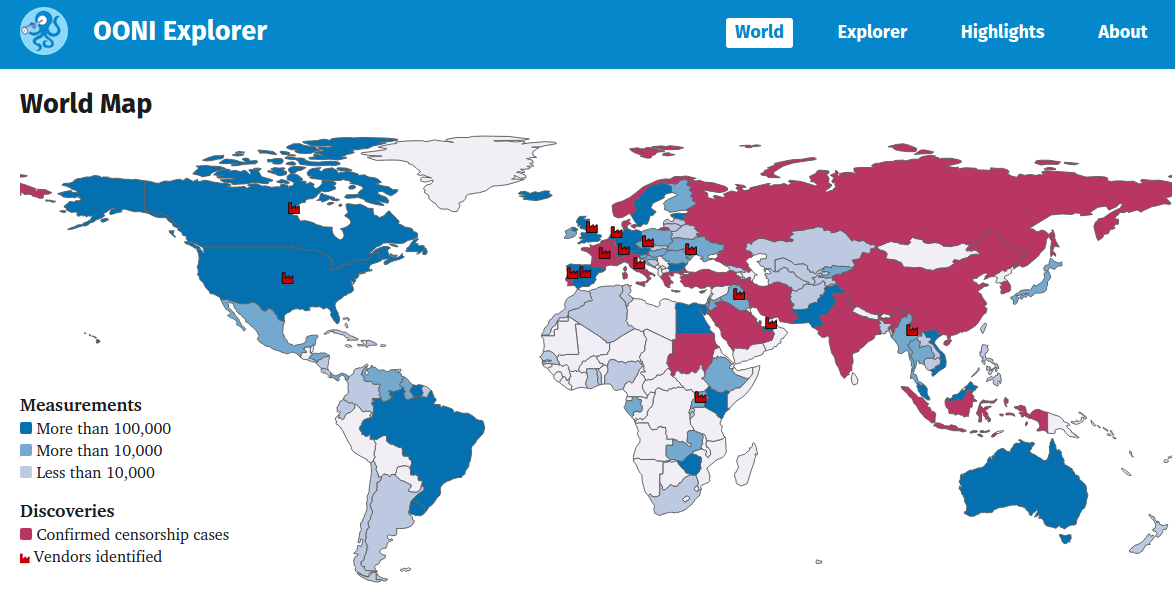
\includegraphics[width=1.0\textwidth]{fig/ooni_map.png}
    \caption{Tor's OONI project collects censorship event data.}
    
    \label{fig:oonimap}
\end{figure*}
%%%%%%%%%%%%%%%%%%%%%%%%%%%%%%%%%%%%%%%%%%%%%%%%%%%%%%%%%%%%%%%%%%%%%%

In our proxy distribution problem, we accept that proxies will be distributed to censors. Our goal is to provide service to clients while preserving some proxies from distribution. In this thesis, we introduce a lightweight approach for the proxy distribution problem to distribute proxies to clients while fake clients are present. We implement a scheme with the goal to maximize the resource loss of an attacker. Our approach uses principles of load balancing in a non-intuitive way to preserve random proxies by unbalancing the load on proxies, making them more difficult to discover. This approach operates on the pessimistic assumption that all proxies are destined for discovery over time in a system, where the system cannot distinguish between honest users and fake users. 
We provide an approximation of the censor's required effort to discover all of the proxies in a system based on the coupon collector problem\cite{flajolet1992birthday}. We validate this approach in a simulator that simulates a proxy distributor in a censorship resistance system. 

We offer a lightweight solution to the proxy distribution problem by slowing down the progress of the censor to learn new proxies. We contribute to the existing body of knowledge in the following five ways:
\begin{enumerate}
    \item We introduce a novel algorithm, \emph{needle}, that uses reversed power of two choices and uniform random batched distribution to slow the expected time of proxy system compromise.
    \item We analyze the needle algorithm in the context of the coupon collector problem to give bounds on the average time to collect all of the proxies.
    \item We define a censorship threat model to evaluate the needle algorithm in proxy distribution. We define honest users, a proxy distributor, insider attackers, and a colluding censor within this model.
    \item We build a simulation to evaluate the needle proxy distribution algorithm and use this to compare the results of the needle algorithm with Tor's \texttt{bridgedb} distribution, general uniform random and power of two choice load balancing algorithms. 
    \item We discuss the benefits and drawbacks of trust-based proxy distribution vs. lightweight approaches and provide ideas for future work on our approach.
\end{enumerate}
\chapter{Background}
\label{sec:background}
\newtheorem{theorem}{Theorem}

\section{Censorship Threat Model} 

The first goal of our censor in this model is to discover proxies. The censor discovers, or \textit{enumerates}, proxies by posing as a legitimate user of a \ac{CRS}. The distribution of proxies to honest users and the censor posing as an honest user is a cat-and-mouse game between the censor and a \ac{CRS}, referred to as the \textit{proxy distribution problem}. 

There are three attacks that lead to the ability of our censor to block a proxy; the Sybil attack followed by the insider attack leading to the enumeration attack. In the first stage of the insider attack, a malicious entity, such as a censor, deploys multiple accounts through anonymous authentication. This is the \textit{Sybil attack} that creates fake accounts to gain entry to the system. The \textit{insider attack} occurs when the knowledge of assigned proxies gained from honest proxy assignment is given to the censor. The \textit{enumeration attack} that follows is usually the action of the censor to block all of the proxies it knows about \cite{wang2013rbridge}.

Once a censor knows about a proxy, it can decide to block that proxy. The second goal of our censor is to block the largest amount of honest users as possible. The censor may choose to block immediately when a proxy is discovered, known as \textit{immediate blocking}. The censor may instead \textit{delay blocking} in order to maximize the collateral damage to honest clients, or perhaps wait for  a critical time or maximum number of users to time a blocking attack. 

In addition, the censor keeps track of proxies that are the most \textit{popular}. The censor determines that a proxy is popular by the number of times a proxy is assigned compared to other proxies that it knows about. The censor then chooses to block proxies based on their popularity ranking.

We make different kinds of blocking assumptions in the evaluation section in Chapter \ref{sec:eval}. Immediate blocking makes the most sense when we evaluate enumeration because as soon as the censor is assigned to any proxy, it is enumerated. We assume delayed blocking behaviour in the load balancing analysis because we want to observe load balancing trends over time, without any blocking on the part of the censor. The bystander evaluation assumes that the censor blocks the most popular proxies so that we can measure the number of bystanders in the remaining proxies.

\subsection{Out of Scope}

The censor is a powerful, nation-state adversary and many of its capabilities are beyond the scope of this work. For example, network-level proxy discovery where the censor actively or passively scans \ac{IP} addresses is not addressed. A censor may monitor all traffic in their network, store the state of the network, and monitor requests and responses to known proxy addresses. This allows the censor to potentially mount a zig-zag attack to connect users together by their proxies \cite{BRIDGEDISCO:2019}. Only proxy discovery by assignment of an attacker to a proxy is explored in this thesis.

\section{Coupon Collector Problem}

In our model, the problem of proxy distribution is simply to distribute a collection of $n$ proxies to some users, where $k$ of these users are attackers, in such a way as to provide a degree of functionality to the honest users. From the censor's viewpoint, it closely aligns to the \ac{CCP} where the proxies are coupons and the censor is the coupon collector.

\ac{CCP} is a classic occupancy problem that considers the number of coupons that must be collected before one has the entire collection of coupons. There are $n$ distinct coupons that are collected one at a time where the $i^{th}$ coupon arrives with probability $p_i$ \cite{motwani1995randomized}. The uniform random algorithm, shown in Algorithm \ref{uni}, chooses one coupon randomly from the list of total coupons.

Where probabilities $p_i$ from $i=1$ to $n$ are equal, the arrivals are uniform random. This equi-probable case, where all probabilities of coupons are equal, shows that the probability of obtaining a new coupon $i$ decreases with each draw. The average number of draws to collect all of the coupons is $nH_n$ where $H_n$ is the $n^{th}$ harmonic number \cite{flajolet1992birthday}. We briefly show why this is the case below. 

The summation of probabilities of obtaining a distinct coupon, not previously seen, is $\frac{n}{n} + \frac{n-1}{n} + \frac{n-2}{n} + ... + \frac{1}{n}$. The probability of receiving a unique coupon decreases by $1$ in the numerator for each selection. The probability of a new coupon in the first draw is $100\%$ for instance, because no coupon has yet appeared. The very last coupon is the most difficult to select with probability = $1/n$.
By linearity of expectations, where $p_i$ is the probability of obtaining the $i^{th}$ coupon, this can be written as:

$$p_i = \sum_{i=0}^{n-1}\frac{n-i}{n}$$

This follows a geometric distribution, therefore $E[X_i]=\frac{1}{p_i}$ where $X$ is the sum of the expected number of draws for the $i^{th}$ coupon from $i$ to $n$.
%\ivan{What about $X_i$ -- how is it related to $X$?}
%\ivan{Make sure to define the variables before you use them in derivations (e.g., $X_i$ here).}
The expected number of draws for all $n$ coupons in total is:

$$E[X] = \sum_{i=0}^{n-1}\frac{n}{n-i}$$

By changing the variable $i$ to $j=n-i$, we obtain $E[X] = nH_n$, where $H_n$ is the $n^{th}$ harmonic number:

$$E[X] = n \sum_{j=1}^{n}\frac{1}{j}$$
$$= nH_n$$

\begin{algorithm}[t]
\DontPrintSemicolon
\KwData{A list of coupons and one randomly selected coupon $c$. Coupons are selected uniform randomly}
\KwResult{A coupon $c$}
\Begin{
    $c \longleftarrow$ random$(coupons)$\;
}
\caption{Uniform Random Coupon Collection \label{uni}}
\end{algorithm}

We use two previous works in our analyses in Chapter \ref{sec:analysis}; the uniform random approximation and singleton coupons.

\subsection{Harmonic Number Approximation} 

Recall that the censor collects $n$ proxies in $E[X]= nH_n$ steps. There is no closed form expression for the harmonic number, $H_n$. Instead, the approximation with Euler Mascheroni Constant $\gamma \approx 0.5772156649$ and $H_n = \ln{n} + \gamma + 1/2n$ is used in this analysis \cite{flajolet1992birthday}.
% TODO is this better than n \ln n? I've also seen that around.

\subsection{Singleton Coupons} 

Variations of the \ac{CCP} are explored in \cite{myers2006some} where a single collector attempts to obtain a specific number of coupons out of $n$ total coupons. As part of this analysis, we use the number of singleton coupons that Myers et al. provide. Singleton coupons are coupons that have been selected exactly once after all of the other coupons have been collected. Most coupons are duplicates and only a few appear only once. On average, the number of singleton coupons is equal to the harmonic number $H_n$.

\section{Load Balancing} 

From the perspective of the proxy distributor, the proxy distribution problem is a form of load balancing where some clients are malicious and the proxy distributor would like to allocate as many proxies as possible to honest clients. Load balancing strategies are used to evenly allocate resources in distributed systems and have historically been modelled as balls and bins \cite{mitzenmacher2005probability}. 

\subsection{Maximum Load}

The evenness of the distribution is formalized as the \textit{maximum load}. The maximum load is equal to the number of balls in the bin that has, with high probability\footnote{with high probability means at least $1 - O(1/n)$}, the maximum number of balls over all the bins. The closer that the maximum load is to a perfect distribution of $m$ balls over $n$ bins, $m/n$, the more even the distribution, and thereby the load is more evenly balanced. 

\subsection{Uniform Random Distribution} 

The maximum load of a uniform random placement of balls in bins where $m=n$ is well known to be approximately $\log n / \log \log n$ with high probability \cite{gonnet1981expected}.
See Lemma 5.1 below from the analysis in Chapter 5 of \textit{Probability and Computing} \cite{mitzenmacher2005probability}. 

\newtheorem{lemma}[theorem]{Lemma}

\begin{lemma} When n balls are thrown independently and uniformly at random into n bins, the probability that the maximum load is more than $3 \ln n / \ln \ln n$ is at most $1/n$ for $n$ sufficiently large.
\end{lemma}


\subsection{Power of 2 Choice} 

The \emph{power of 2 choice} algorithm for load balancing shows that giving two random choices instead of a uniform random placement results in an exponential improvement in the maximum load \cite{mitzenmacher1996power}. Figure \ref{POD} outlines the power of 2 choices algorithm that randomly selects two bins from the total list of bins. To determine the bin that is selected, the algorithm checks the load of each bin. The bin with the \emph{least} number of client assignments is returned. 

\begin{algorithm}[t]
\DontPrintSemicolon
\KwData{A list of bins $bins$, two randomly selected bins $b_1$ and $b_2$ with total number balls, or loads, $l_1$ and $l_2$ respectively}
\KwResult{One of $\{b_1, b_2\}$}
\Begin{
    $b_1 \longleftarrow$ random$(bins)$\;
    $b_2 \longleftarrow$ random$(bins)$\;
    $l_1 \longleftarrow$ $load(b_1)$\;
    $l_2 \longleftarrow$ $load(b_2)$\;

    \uIf{$l_1 == l_2$}{
        return random$(b_1, b_2)$\;\tcc*[r]{break a tie}
    }
    \uElseIf{$l_1 < l_2$}{
        return $b_1$\;\tcc*[r]{$b_1$ is least loaded}
    }

    return $b_2$\;\tcc*[r]{$b_2$ is least loaded}
}
\caption{Power of Two Choices \label{POD}}
\end{algorithm}

The maximum load in the uniform random case is $\frac{\log n}{\log \log n} + O(1)$ where the number of balls is equal to the number of bins \cite{azar1999balanced}. In the two-choice algorithm, the fullest bin with high probability has $ \frac{\log \log n}{\log 2} + O(1)$ balls where the number of bins selected randomly is $2$. Increasing the number of bins $\geq 2$ yields only a constant factor of improvement. The heavily loaded case, where the number of balls strictly increases over the number of bins, $m >> n$, was found to have a maximum load of $m/n + O(\log{\log{n}})$ \cite{berenbrink2000balanced}. \\

\section{Tor} 

One of the most widely used distributed, anonymous networks is the Tor onion network. Tor is useful for avoiding traffic analysis, a form of internet surveillance, but any anonymous network on its own is insufficient for censorship circumvention. For example, Tor packets are identifiable from telltale signs in the format of traffic sent to the Tor network. Additionally, these packets are easily blacklisted by censors because onion relay \ac{IP} addresses in the onion network are publicly known. Tor includes various obfuscation protocols, known as \texttt{pluggable transports}, to hide distinguishing characteristics of packets from censors. These protocols are run by Tor \texttt{bridges}; bridges are single-hop proxies into the Tor onion network. Bridges are run by volunteers in a trusted proxy environment outside of the censor boundary. Tor needs to communicate the address of a bridge to legitimate users securely. This is another form of the proxy distribution problem; to distribute secret bridge addresses (proxies) only to legitimate users, not to censors. 

A user requests bridge addresses from Tor by emailing Tor's bridge service. The bridge service, \texttt{bridgedb}, selects three bridge addresses at a time and rate limits these requests. For example, a request from a single email address can request bridges once daily. The \texttt{bridgedb} data structure is a hashring where an index into the keyspace is generated by hashing unique user information into a subring that is rotated on a scheduled interval.\footnote{https://gitweb.torproject.org/bridgedb.git/tree/bridgedb/distributors/email/distributor.py} This index gives the first bridge address, the other two bridge addresses are the successors of the first index in the ring. The censor can enumerate bridges one-by-one by posing as a legitimate user. Ling, Luo, Yu, Yang, and Fu showed in \cite{ling2015tor} that Tor bridges can be enumerated with bulk emails via the \ac{HTTPS} protocol.\\

Coming up next, in Chapter \ref{sec:analysis}, we'll analyze the expected time to collect all of the proxies using the needle algorithm in the context of the coupon collector problem. We'll also refer to the maximum load in the load balancing analysis. Later on, in Chapter \ref{sec:eval}, we'll compare the uniform random, power of 2 choices, and Tor's distribution mechanism with the needle algorithm in our evaluation.
\chapter{Needle Algorithm}
\label{sec:analysis}

\begin{algorithm}[t]
\DontPrintSemicolon
\KwData{$proxies$, $n$, $s=\lfloor{n/g}\rfloor$}
\KwResult{One of $\{px_1, px_2\}$}
\Begin{
    $window \longleftarrow (start, end)$\;
    \uIf{$move > 1$}{
        \tcc*[l]{a giant step around the proxy ring}

        $start \longleftarrow (start + s)$ \% $n$\;
        $end \longleftarrow (end + s)$ \% $n$\;
        $move \longleftarrow 0$
    }
    
    $move \longleftarrow move + 1$\;
    
    $sublist \longleftarrow (proxies$ $[start, end])$\;

    $px_1 \longleftarrow$ random$(sublist)$\;
    $px_2 \longleftarrow$ random$(sublist)$\;
    $l_1 \longleftarrow$ $load(px_1)$\;
    $l_2 \longleftarrow$ $load(px_2)$\;

    \uIf{$l_1 == l_2$}{
        return $px_1$\;\tcc*[r]{break a tie}
    }
    \uElseIf{$l_1 > l_2$}{
        return $px_1$\;\tcc*[r]{$px_1$ is heaviest loaded}
    }
    return $px_2$\;\tcc*[r]{$px_2$ is heaviest loaded}
    
}
\caption{Needle Algorithm \label{needle}}
\end{algorithm}

I present a new algorithm, the \emph{needle} algorithm, and compare it to two well-known algorithms, uniform random and power of 2 choices, as well as Tor's bridge distribution scheme, in order to contrast their respective trade-offs and suitability under differing system goals. The goal of the needle algorithm is to preserve some proxies from within the larger list of $n$ proxies. It achieves this by breaking the list of proxies into sublists. It moves through the proxies jumping from sublist to sublist, referred to as \texttt{GIANTSTEPS} or $g$. These steps isolate some proxies from distribution.\footnote{Those readers familiar with the algorithmic composition techniques of jazz chord progression may draw a parallel from the restriction of proxies to the restriction of notes in a key change. These are reminiscent of Coltrane's Giant Steps \cite{lateef1981repository}.} The algorithm has the following parameters:
    \begin{itemize}
        \item $proxies$: a sorted list of proxies ordered by load
        \item $n$: the total number of proxies
        \item $g$: the number of steps around the proxy ring
        \item $s$: the number of proxies in each $g$ step
        \item $move$: move to the next step 
        \item $px_1, px_2$: two randomly selected proxies from within the $sublist$ of the current step $g$, sampled with replacement
    \end{itemize}

The algorithm selects two proxies uniform randomly in each giant step $g$. Using reverse power of 2 choices, it then chooses the \textit{heavier loaded} proxy and returns this proxy to the collector. (Note that the standard power of d choices algorithm chooses the lighter loaded proxy.) The step begins at the bottom of the list of proxies and is moved step-wise around the list eventually wrapping so that all proxies have an opportunity to be selected, shown in Figure \ref{fig:giantstepring}.

%%%%%%%%%%%%%%%%%%%%%%%%%%%%%%%%%%%%%%%%%%%%%%%%%%%%%%%%%%%%%%%%%%%%%%
\begin{figure*}[h!]
\centering
     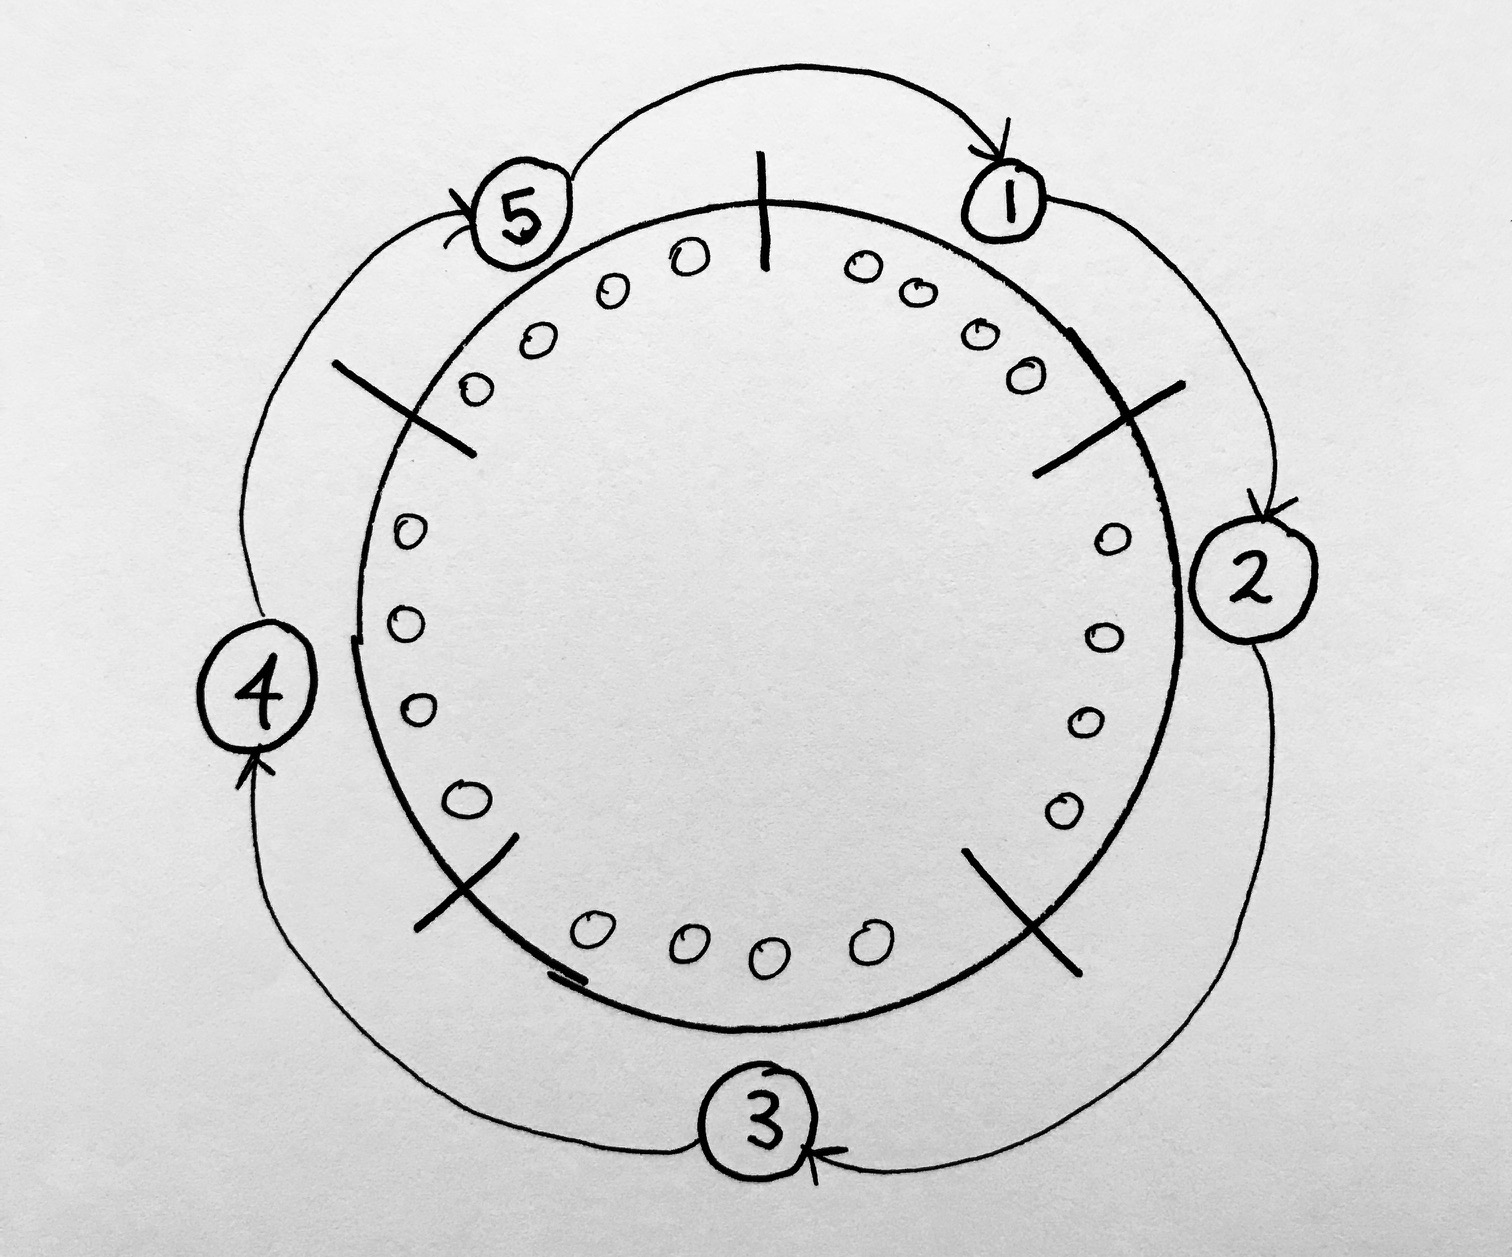
\includegraphics[width=0.5\textwidth]{fig/giant_step_ring.png}
    \caption{$5$ giant steps around a ring of $20$ proxies}

    \label{fig:giantstepring}
\end{figure*}
%%%%%%%%%%%%%%%%%%%%%%%%%%%%%%%%%%%%%%%%%%%%%%%%%%%%%%%%%%%%%%%%%%%%%%

Some number of proxies are less likely to be selected as step $g$ moves. For example, the proxies in previous selections left behind are referred to as \emph{needles} because they are hidden from the current selection. Additionally, proxies that have a lower chance of appearing in the random selection, e.g., the last few distinct proxies to be selected, have a lower probability of appearing in any selection. As $g$ moves, it also unbalances the load on proxies thereby increasing the number of selections that the censor must perform because there are more duplicate selections (misses).
\section{Coupon Collector Variant: Neighbourhood Ring}

One may find a parallel between the Coupon Collector Problem (CCP) and the problem of a censor who collects, not coupons, but proxies. Consider both the coupon and proxy as objects in some vast space, where all of these objects have the same chance of being selected. Each object is replaced after it is selected so that any object may be selected multiple times. It is increasingly difficult to collect a distinct object because most objects are selected more than once. The rarest object is the one that occurs at the very end to complete the collection. The selection of this very last unique object ends the game, since only the selection of distinct objects counts towards progress in this problem.

We can frame the needle algorithm as a CCP variant. Suppose that the coupon collector organizes collections from several different neighbourhoods. Each neighbourhood distributes a different set of coupons, and each of the coupons in each set is distinct. The coupon collector needs to travel through all of the neighbourhoods (these are conveniently arranged in a ring). The collector can't magically move from place to place and does not zigzag from neighbourhood to neighbourhood. If the collector misses a coupon from the first neighbourhood, then he must wait until all of the other neighbourhoods are visited before returning to collect the missed coupon. The missed coupon is rarer than all of the previously collected coupons. It is also rarer than all future coupons up until the point at which the collector returns to the specific neighbourhood with the missed coupon.

In our CCP variant, the reverse power of 2 choices gives the collector a decision to make; he selects 2 coupons at random. If he already has more of 1 coupon than the other, he must keep the coupon that is less rare, and return the rarer coupon back to the store in the current neighbourhood. 

There is an expected number of attempts $E[X]$ by the collector to collect $n$ distinct objects. This can be extended to a censor, whose problem it is to enumerate, or discover, all the proxies. We use $E[X]$ to analyze the amount of effort that it would take a censor, on average, to enumerate all proxies. To simplify this analysis, we do not consider the ratio of honest to malicious clients and, for now, assume there is one malicious client, the censor. Honest and malicious client rates are examined in Section \ref{sec:bystander}, bystanders.

The needle algorithm is partly randomized and partly deterministic. The uniform random selection of 2 proxies is randomized, and the reverse power of 2 choices is deterministic. In addition, the movement of the steps is also deterministic. Because the steps move clock-wise around the ring, proxies are enumerated randomly within deterministic batches. Moving the steps around the ring serves two functions; 1) by limiting the size of proxies in a step, it squeezes the number of possible proxies that a censor can enumerate in each assignment, and 2) some proxies are left behind. This makes it more difficult for the censor to enumerate a complete collection of proxies due to these rare proxies (not unlike needles in a haystack). Restricting the size of the sublists in a step tends towards a deterministic enumeration of all of the proxies, so one must take care to not set too many giant steps. 

In Figure \ref{fig:8ring}, we see how different step sizes affect the enumeration of proxies. With one-step, the enumeration time is the slowest, because the needle proxies must be discovered within the largest pool of size $n$. Enumeration time starts to decrease with 2-steps, because the needle proxies are more likely to be selected with a smaller pool size of $n/2$. The enumeration time decreases with each increase in giant step $g$. The algorithm only functions as expected up to $g=n/2$ where there are at least $2$ proxies for each step. If there is only a single proxy in each step, as shown in the bottom right corner, the proxies are enumerated one after the other in $n$ assignments, because our reverse power of 2 choices algorithm cannot function as intended. We therefore restrict the giant step size to $1>g\leq \frac{n}{2}$ so that the proxies are never enumerated in deterministic order.

%%%%%%%%%%%%%%%%%%%%%%%%%%%%%%%%%%%%%%%%%%%%%%%%%%%%%%%%%%%%%%%%%%%%%%
\begin{figure*}[h!]
\centering
     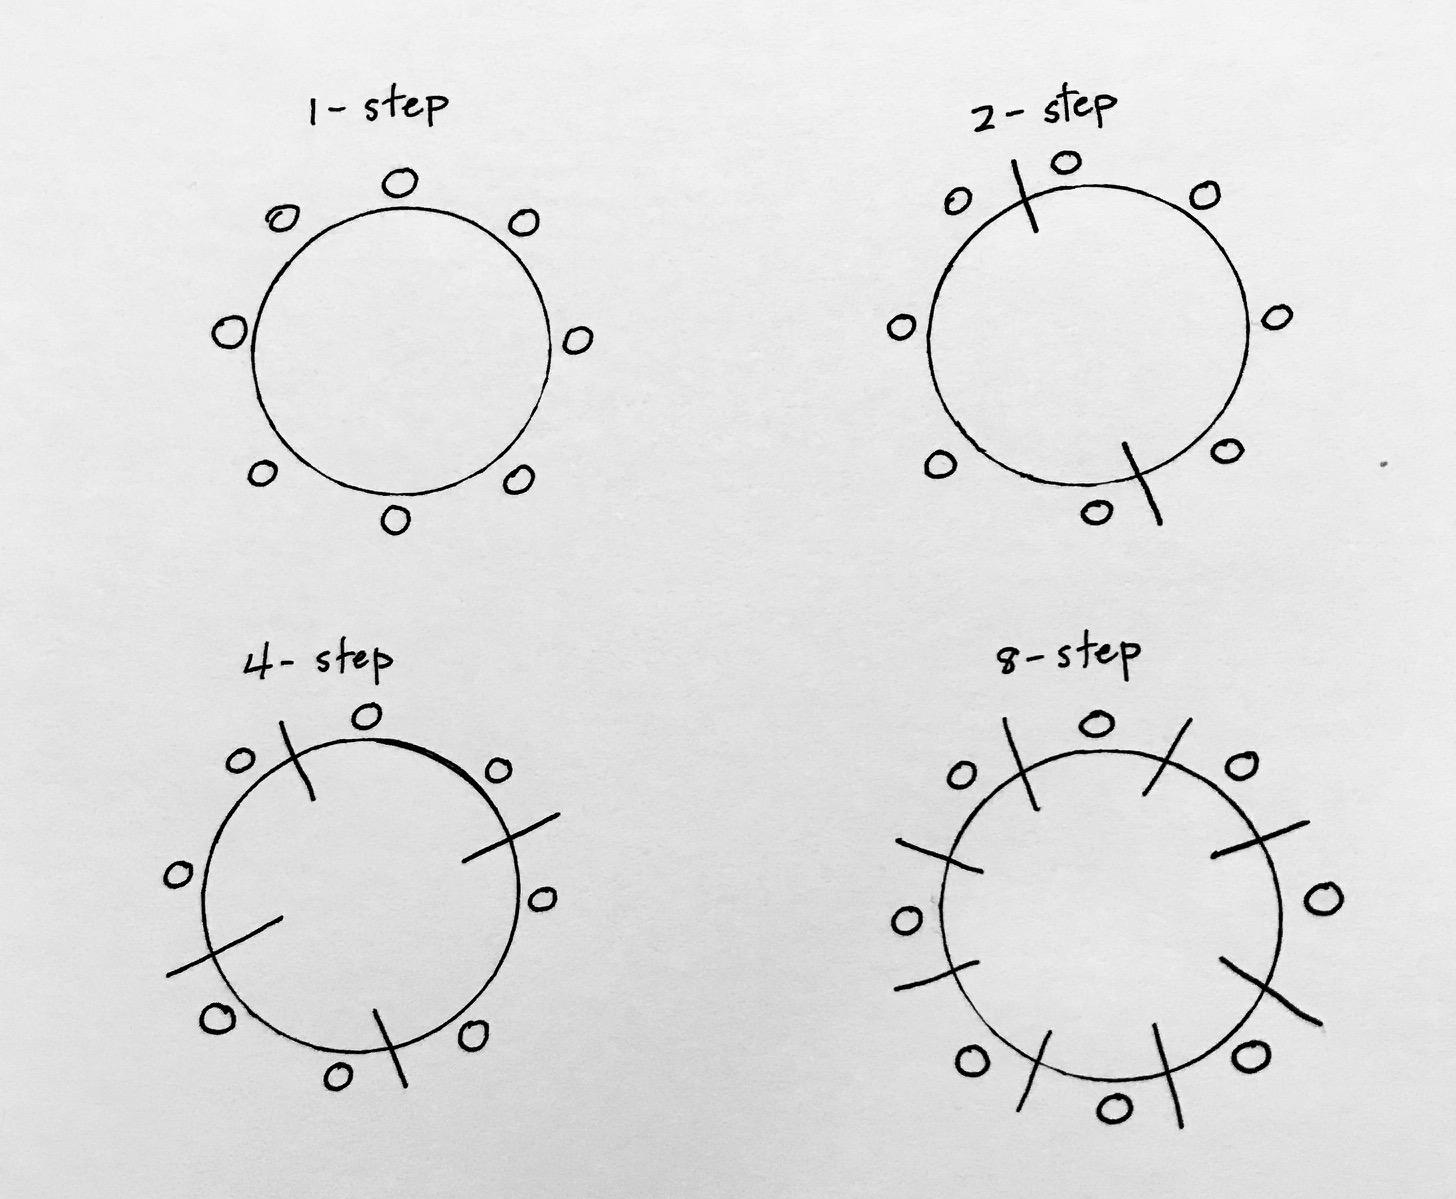
\includegraphics[width=0.5\textwidth]{fig/8_ring.png}
    \caption{Ring of 8 proxies with steps g=1,2,4,8}

    \label{fig:8ring}
\end{figure*}
%%%%%%%%%%%%%%%%%%%%%%%%%%%%%%%%%%%%%%%%%%%%%%%%%%%%%%%%%%%%%%%%%%%%%%
 
\section{Enumeration Analysis}

Recall that the enumeration of our collection of proxies occurs when the censor learns all of the proxies through assignment. The enumeration of proxies is modeled as the complete collection of coupons. The CCP neighbourhood ring variant is used to calculate the average time to collect all distinct proxies.
 

\begin{table}[h]
  \centering
	\begin{tabular}{ll}
	\hline
	\cline{1-2}
	Parameter Name    & Description  \\
	\hline
    $n$     & total number of proxies \\
	$g$     & number of steps around a proxy ring  \\
	$s$     & size of proxies allocated in each step $n/g$ \\
    $H_n$   & harmonic number \\
    $px_i$  & the $i^{th}$ proxy \\
    $p_i$   & probability that the $i^{th}$ proxy is enumerated \\
    $p$     & sum probability that proxies $1$ to $n$ are enumerated \\
    $X_i$   & random variable of assignments to enumerate the $i^{th}$ proxy \\
    $X$     & random variable of sum of $X_i$ from $1$ to $n$ \\
    $E[X]$  & expected time on average to enumerate all proxies \\
	\hline
	\end{tabular}
  \caption{Notation used in the Enumeration Analysis}
  \label{tab:vars}
\end{table}

There are two different, yet intertwined, flavours of probabilities in our algorithm; the probability of \textit{selection} and the probability of \textit{choice}. The probability of selection is uniform random and is restricted by the size of the giant step $g$. When a pair of proxies is selected uniform randomly from the total collection of proxies, this is referred to as the selection. When we refer to likelihood of selection, we are talking about the probability of selection in relation to the coupon collector problem. Because we sample proxies randomly with replacement, a proxy can be selected twice in a pair. The probability of choice relates to the order in which a proxy is selected as a pair. The likelihood of choice is dependent on the load of a proxy as it affects the choice in the reverse power of 2 choices algorithm. Probability of choice is important in our analyses, particularly in the load balancing analysis.

\subsection{Algorithm Termination}

We define two lemmas below that we will use to approximate upper and lower bounds on the average enumeration time. We define the algorithm termination in terms of the rarest proxy, the last distinct proxy that is selected, $px_n$. Proxy $px_n$ has the probability of selection = $1/n$ making it the rarest proxy out of all of the other proxies. Note that this proxy must have load = 0 because it was never previously chosen out of a selected pair. Recall that the reverse power of 2 algorithm chooses the proxy with the highest load out of a pair of proxies. The rarest proxy can only be chosen if it is compared against itself. The only case where this occurs (when the proxy appears with probability of selection $1/n$) is when this proxy is selected in a pair. 

\begin{lemma}{A pair of the rarest proxy terminates the algorithm.}
\label{rarest}

Assume we have the rarest proxy \textbf{$px_n$} that has probability equal to $1/n$ of being selected in the reverse power of 2 choices algorithm. Suppose that this proxy is selected twice in a row and forms a pair. If the choice from this selected pair does not terminate the algorithm, there must be some other proxy in the collection of $n$ proxies that has not yet been chosen. If this statement is true, then proxy \textbf{$px_n$} must have a probability greater than $1/n$ and our initial assumption is false, leading us to a contradiction. Therefore, the proxy with probability $1/n$ terminates the algorithm if it is selected twice in a row, as a pair. In other words, the least likely, rarest proxy must occur as a pair for the algorithm to terminate. 
\end{lemma}

\begin{lemma}{The probability of enumerating the rarest proxy is at least $1/n^2$.}

By Lemma \ref{rarest}, the needle algorithm terminates after the rarest proxy is selected in a pair. The probability that the rarest proxy is selected is $1/n$. We sample with replacement, so the probability that the rarest proxy is selected twice in a pair, by counting argument, is $p=(\frac{1}{n})(\frac{1}{n}) = 1/n^2$.
\end{lemma}

\subsection{Upper Bound}  

We use the number of singletons described in Chapter \ref{sec:background}, $H_n$, directly to provide an upper bound on the average number of pairs selected, $E[X]$, before all of the proxies are enumerated. Singletons are proxies that occur only once and so have the lowest probability of selection. These proxies need to be paired with other proxies that have lighter loads to ensure that they are chosen by the reversed power of 2 choice algorithm. (They also need to appear as the first item in the pair for the tie-breaking logic.) Most of the singleton proxies occur at the end of the selection process, so the probability of selection for each of them is closer to $1/n$ than $n/n$. In the worst case (for the censor), all of the singleton proxies occur at the end of the collection. Since most of the proxies have load $> 1$ as $n$ increases, there is little chance that singleton proxies are chosen against non-singleton proxies, because most of these non-singleton proxies have appeared numerous times already and have higher assignment loads.

\begin{lemma}{The probability of collecting all of the singleton proxies is \\
$$\sum_{i=1}^{\lceil{H_n}\rceil} \bigg(\frac{i}{n^2}\bigg)$$}

The probability of collecting all of the singleton proxies is bounded above by the likelihood that the singleton proxies are selected in a pair with the rarest proxy $px_n$, the worst case for a censor. The rarest proxy $px_n$ is selected with probability $\frac{1}{n}$. The probability that some $i^{th}$ singleton proxy is selected in a pairing with $px_n$ is $p_i = (\frac{i}{n})(\frac{1}{n})$. 

If we pair all of the singleton proxies with the rarest singleton proxy, $px_n$, we get the probability pairs $(\frac{1}{n})(\frac{1}{n}) + (\frac{2}{n})(\frac{1}{n}) + ... + (\frac{H_n}{n})(\frac{1}{n})$. There is no guarantee that $H_n$ is an integer, indeed it will not be. Fractional pairings can't happen in our pairings, e.g. there is no half of a proxy selected. Because we are dealing with an upper bound, we say that the number of singleton proxies is $\leq \lceil{H_n}\rceil$. In addition, we need an even number of pairings, so $\lceil{H_n}\rceil$ is rounded to an even number. Generally stated, the probability of this pairing over all $H_n$ singletons is:

$$p \leq \sum_{i=1}^{\lceil{H_n}\rceil} \bigg(\frac{i}{n}\bigg) \bigg(\frac{1}{n}\bigg)$$
$$= \sum_{i=1}^{\lceil{H_n}\rceil} \bigg(\frac{i}{n^2}\bigg)$$

\end{lemma}

Now, we are ready to present the upper bound on the average number of assignments before all of the proxies are enumerated. Recall that $X_i$ is a random variable representing the number of assignments needed to enumerate the $i^{th}$ proxy, therefore $E[X_i]$ is the average number of assignments to collect the $i^{th}$ proxy. $E[X]$ is the average number of assignments needed to enumerate all of the proxies. We denote the $i^{th}$ proxy as $px_i$ where the last selected, rarest proxy is $px_{n}$ with probability $1/n$. The second rarest proxy is $px_{n-1}$ with probability $2/n$. The first proxy selected is $px_1$ with probability $1$.\\
 
\label{theorem:UBEX}
\begin{theorem} {Upper bound on $E[X] \leq \frac{n^2H_{\lceil{H_n}\rceil}}{g}$} 
\end{theorem}

\emph{Proof.} We use the probability of collecting all of the $H_n$ singleton proxies from Lemma $4$ to provide an upper bound on the average number of assignments needed to enumerate all of the proxies, $E[X]$. 

Like the classic CCP, this follows a geometric distribution, so $E[X_i] =\frac{1}{P_i}$. 

$$E[X_i] = 1/p_i = \frac{1}{\frac{i}{n^2}} = \frac{n^2}{i}$$

The expected number of assignments to find all $n$ proxies is bounded above by the sum of $E[X_1]$ to $E[X_n]$, where $n=\lceil{H_n}\rceil$:\\

$$E[X] \leq \sum_{i=1}^{\lceil{H_n}\rceil} \bigg(\frac{n^2}{i}\bigg)$$
$$E[X] = n^2 \sum_{i=1}^{\lceil{H_n}\rceil} \bigg(\frac{1}{i}\bigg)$$
$$E[X] = \bigg(n^2\bigg) \bigg(H_{\lceil{H_n}\rceil}\bigg)$$

When giant step $g$ is very small, the algorithm churns on a few proxies, meaning that a small proportion of proxies have high loads. By dividing $n$ proxies into $g>1$ giant steps, where each step has a sublist of size $s$, we make the algorithm more load balanced. In other words, the distribution of proxies in each step is smaller so the censor gets more chances to find the singletons.  We rework the upper bound to incorporate the number of giant steps $g$.

%%%%%%%%%%%%%%%%%%%%%%%%%%%%%%%%%%%%%%%%%%%%%%%%%%%%%%%%%%%%%%%%%%%%%%
\begin{figure*}[h!]
\centering
     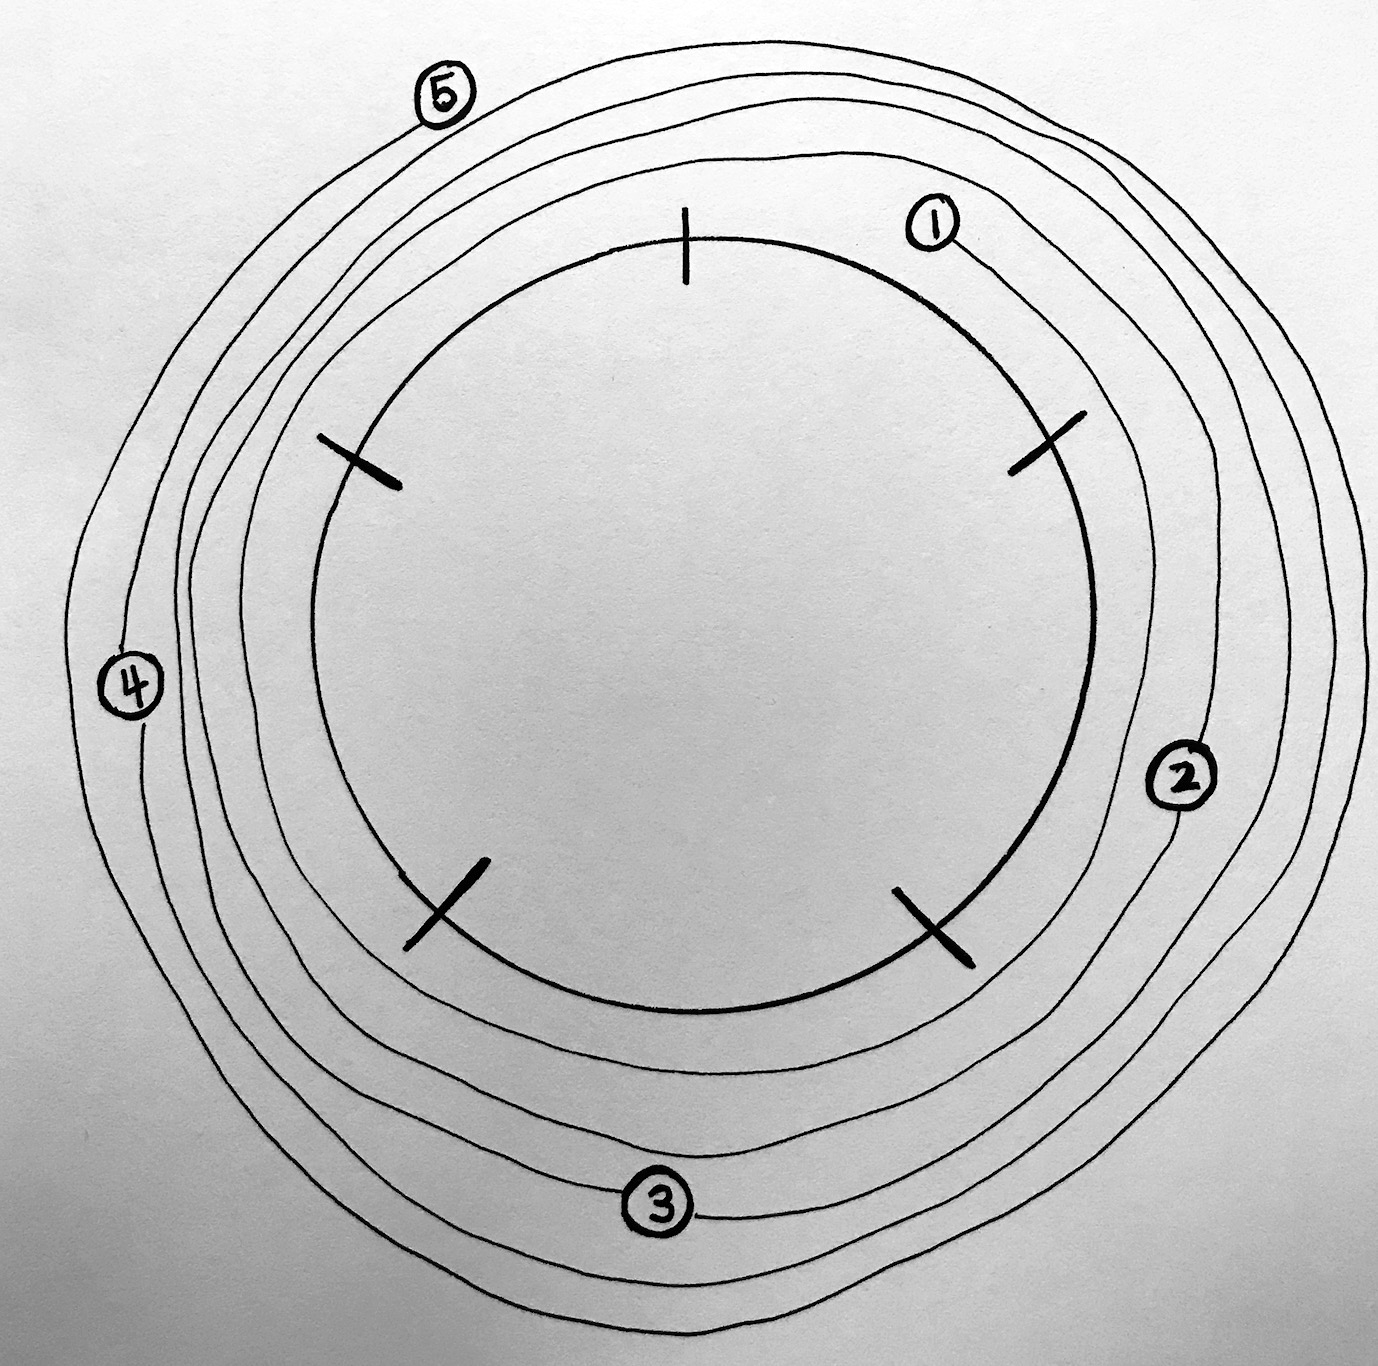
\includegraphics[width=0.5\textwidth]{fig/giant_step_upper_bound.png}
    \caption{Worst case enumeration in $5$ giant steps.}

    \label{fig:ubgs}
\end{figure*}
%%%%%%%%%%%%%%%%%%%%%%%%%%%%%%%%%%%%%%%%%%%%%%%%%%%%%%%%%%%%%%%%%%%%%%

We have $g$ giant steps and $H_n$ singleton proxies; $g$ divides the enumeration time into smaller sized sublists, making it proportionally easier for the censor to enumerate all $n$ proxies. In the worst case (for the censor), all of the singleton proxies are located in different steps, so all of the steps wait for the other steps' singletons to be enumerated before the algorithm can terminate. Figure \ref{fig:ubgs} shows a collection of proxies with $5$ giant steps. The first enumerated sublist occurs in the top right portion of the ring (denoted $(1)$). The algorithm proceeds clock-wise, moving through each sublist one by one. We divide the upper bound by the number of steps $g$ to obtain:

$$E[X] \leq \frac{ n^2H_{\lceil{H_n}\rceil}}{g}$$


\subsection{Lower Bound}
Before we present the lower bound on the average number of assignments before all of the proxies are enumerated, we consider the probability of singleton proxies that are very likely to be chosen. The reverse power of 2 choices relies on the load of the proxy in order to choose a proxy from a selected pair. Consider a singleton proxy that by definition has a lighter load because it is selected infrequently. When this proxy is paired with some other proxy with a higher probability of selection, the singleton proxy has \textit{less} chance to be chosen, because the proxy with the higher probability of selection has a higher chance of having more load. In other words, this singleton proxy has both a lower probability of selection and lower probability of choice. 

We concern ourselves with a lower bound, so we would like to know the type of scenario in which a singleton proxy has the higher probability of choice, meaning that the censor is able to enumerate proxies more easily. A singleton proxy paired with itself is guaranteed to be chosen and thus has the highest probability of choice out of any other pairing. We would like to know the probability of a pair of singleton proxies to appear.

\begin{lemma}{Singleton proxies occur in a pair with probability $p \geq \sum_{i=1}^{\lfloor{H_n}\rfloor} (\frac{i}{n})^2$}

% Maybe a bit confusing: 
% Another intuition is to consider the pairing of a singleton proxy with another, rarer singleton proxy because the rarer proxy most likely has a lighter load. This would also result in a high likelihood that the singleton proxy is chosen. However, the probability of selection of this proxy is smaller than the probability of a singleton proxy paired with itself, so it is not useful in developing our lower bound.

A repeated pair selection of the singleton proxies gives us the probability pairs $p=(\frac{1}{n})(\frac{1}{n}) + (\frac{2}{n})(\frac{2}{n}) + ... + (\frac{H_n}{n})(\frac{H_n}{n})$. The probability of the $i^{th}$ singleton proxy to be chosen is $(\frac{i}{n})^2$. The probability of this pairing for all $H_n$ singletons is:

$$p \geq \sum_{i=1}^{\lfloor{H_n}\rfloor} \bigg(\frac{i}{n}\bigg)^2$$

\end{lemma}
%%%%%%%%%%%%%%%%%%%%%%%%%%%%%%%%%%%%%%%%%%%%%%%%%%%%%%%%%%%%%%%%%%%%%%
\begin{figure*}[h!]
\centering
     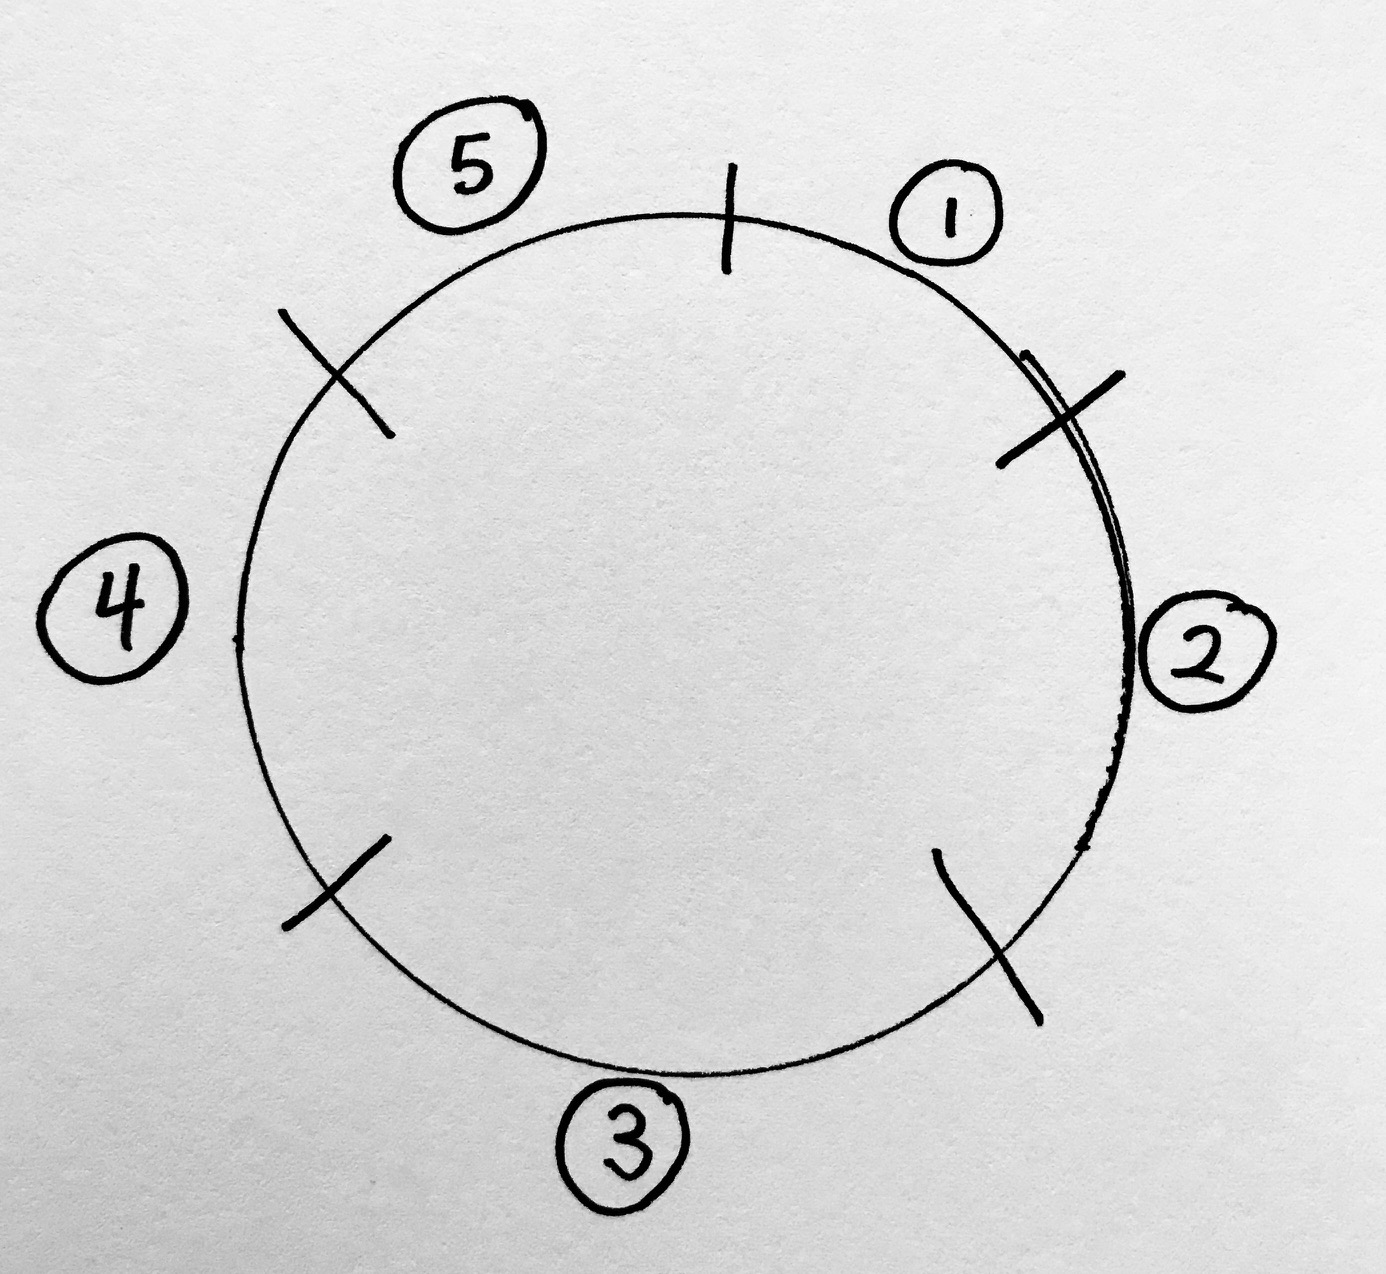
\includegraphics[width=0.5\textwidth]{fig/giant_step_lower_bound.png}
    \caption{Best case enumeration in $5$ giant steps.}

    \label{fig:lbgs}
\end{figure*}
%%%%%%%%%%%%%%%%%%%%%%%%%%%%%%%%%%%%%%%%%%%%%%%%%%%%%%%%%%%%%%%%%%%%%%


We use Lemma $6$ in the following proof to obtain the lower bound on $E[X]$. The fastest enumeration of all of the proxies is to collect all of the singleton proxies the first time that they show up in a randomly selected pair, that is, their very first selection. We again use $H_n$ singleton proxies, this time to bound the average number of assignments from below. We consider cases where $g\geq1$ and we change the variable $n$ to $s$ because we draw from $g$ sublists of size $s$. 

Returning to the idea of a ring of proxies, if all of the sublists are enumerated one directly after the other, none of the other steps are "held up" by any of the other previous steps. This means that there are no extra revolutions necessary to enumerate the steps, as shown in Figure \ref{fig:lbgs}.


\label{theorem:LBEX}
\begin{theorem} {Lower bound on $E[X] \geq (g) (s^2)H^{(2)}_{\lfloor{H_n}\rfloor}$}
\end{theorem}

\emph{Proof.} Using the probability of pairs from Lemma $6$, we have a geometric distribution, so we can write: $$E[X_i] = \frac{1}{p_i} = \frac{1}{(\frac{i}{s})^2} = \bigg(\frac{s}{i}\bigg)^2$$

The expected number of assignments to find all $n$ proxies is bounded below by the sum of $E[X_1]$ to $E[X_n]$, where $n$ is the number of singleton proxies,$n=\lfloor{H_n}\rfloor$:\\

$$E[X] \geq \sum_{i=1}^{\lfloor{H_n}\rfloor} \bigg(\frac{s}{i}\bigg)^2$$
$$= s^2 \sum_{i=1}^{\lfloor{H_n}\rfloor} \frac{1}{i^2}$$
$$= s^2H^{(2)}_{\lfloor{H_n}\rfloor}$$\\

We have $g$ such enumerations of sublists with size $s$, one per each $g$ steps, therefore for all $n$ proxies are bounded from below by:

$$E[X] \geq (g)(s^2)H^{(2)}_{\lfloor{H_n}\rfloor}$$\\

This concludes our discussion of bounds on the average number of assignments to enumerate all of the proxies in the needle algorithm. In the next section, we dive into a load balancing analysis to tell us more about how clients are assigned to proxies.

\label{sec:lb}
\section{Load Balancing Analysis}

We discussed maximum load as a metric for load balancing in Chapter \ref{sec:background}. We cannot guarantee that the number of bins (proxies) is equal to the number of balls (assignments), so the maximum load does not tell the whole picture. We need to look at the least loaded and heaviest loaded extremes and find an average measurement and compare this to the \textit{optimal load}. The optimal load is the load of each proxy if the system was perfectly balanced, that is, if the number of assignments were divided evenly over the number of proxies.

\begin{table}[h]
  \centering
	\begin{tabular}{ll}
	\hline
	\cline{1-2}
	Parameter Name    & Description  \\
	\hline
    $n$     & total number of proxies \\
    $m$     & total number of assignments in a series of trials \\
    $px_i$  & the $i^{th}$ proxy \\
    $p_i$   & probability that the $i^{th}$ proxy is enumerated \\
	$\ell$     & optimal load \\
	$u$     & maximum load \\
    $E[X]$  & expected time on average to enumerate all proxies \\
    $d_1$ & distance between $px_1$ and $px_{\frac{n}{2}}$ \\
    $d_2$ & distance between $px_{\frac{n}{2}}$ and $px_n$ \\
	\hline
	\end{tabular}
  \caption{Notation used in the Load Balancing Analysis}
  \label{tab:vars}
\end{table}

\begin{lemma}{Proxy loads increase linearly.}

We sort the proxies by their load, or their respective numbers of assignments, averaged over multiple trials. (Note that these are not static proxy numbers, but proxies that are numbered by their load.) We see that the loads have a linear relationship. This is because the probability of selection of the $px_i$ proxy decreases linearly from $i=1...n$. The probability of selecting the first proxy $px_1$ is $p_1=\frac{n}{n}=1$, the probability of the second $px_2$ is $p_2=\frac{n-1}{n}$, $p_{n-1}=2/n$, $p_{n}=1/n$, increasing linearly. This linear relationship between the probability of proxy selection is further reinforced by the probability of choice, where the maximum loaded proxy is always chosen over a lower load.
\end{lemma}

\begin{lemma}{The middle proxy, $px_{n/2}$, has the optimal load $\ell$.}

Let the number of total assignments in a series of trials be $m$, and $E[X]$ be the average number of assignments before all proxies are enumerated where $m>>E[X]$. The optimal load is $\ell=m/n$. Proxy $px_{n/2}$ has the probability of selection equal to $p_{\frac{n}{2}}=\frac{n/2}{n}$ in the reverse power of 2 choice selection. It is $n/2$ more likely to be chosen from the selection than proxies $px_1$ to $px_{\frac{n}{2} - 1}$ and $n/2$ less likely to be chosen over proxies $px_{\frac{n}{2} + 1}$. Its placement at the midway point of choice means that it is also at the midway point of the load $\ell$. 
\end{lemma}

\begin{theorem}{The maximum load, $u$, of proxy $px_n$ is twice as big as the optimal load, $2\ell$, if all of the proxies are enumerated.}

We know by CCP that the minimum load is at least $1$ if all of the proxies are enumerated. By Lemma $9$, we see that the middle proxy $px_{\frac{n}{2}}$ has the optimal load. Since the proxy load has a linear relationship by Lemma $8$, the distance, $d_1$ between $px_1$ and $px_{\frac{n}{2}}$ is equivalent to the distance, $d_2$ between $px_{\frac{n}{2}}$ and $px_n$. $px_{\frac{n}{2}}$ has the optimal load and the function is increasing linearly, therefore $px_{n}$ has twice the optimal load $u = 2\ell =(2)(\frac{m}{n})$.

\end{theorem}

\label{sec:bystander}
\section{Bystander Analysis}

Now we consider how honest users are integrated into our analysis where previously we only included the censor's problem of enumerating all of the proxies. We want to know the likelihood that a proxy has been assigned to an attacker, \textit{proxy exposure}, and the proportion of honest users, or \textit{bystanders}, that are affected by proxy exposure.

\begin{table}[h]
  \centering
	\begin{tabular}{ll}
	\hline
	\cline{1-2}
	Parameter Name    & Description  \\
	\hline
    $p_a$       & probability that a client is an attacker\\
    $p_x$     & probability that a proxy is not exposed \\
    $p_e$     & probability that a proxy is exposed \\
	$h$     & historical load on a single proxy  \\
	$\ell$     & optimal load \\
	$u$     & maximum load \\
	$b$     & average number of bystander clients\\

	\hline
	\end{tabular}
  \caption{Notation used in the Bystander Analysis}
  \label{tab:vars}
\end{table}

\begin{lemma}{Proxy Exposure: The probability that a proxy is exposed is greater than $1 - (1-p_a)^{u}$.}

We define an \textit{exposed} proxy as a proxy that has at least one insider attacker assigned at any point in time. In a single assignment of a client to a proxy, the probability that the client is an attacker is given as $p_a$. The total number of assignments in a proxy is equivalent to its load $h$. The probability that \textit{each and every} $h$ client assignments is an attacker is an "and" relationship, so we multiply all of the probabilities of assignment an attacker by the load, $(p_a)^h$. Conversely, the probability that a proxy is \textit{not} exposed i.e. it has not had a single attacker assigned in any of the assignments is:

$$p_x = (1-p_a)^h$$

We can generalize this probability to any proxy in the system using the maximum load bound. Without knowing the load on any individual proxy, we can say that the likelihood that any proxy is not exposed is greater than the likelihood of the maximum loaded proxy $(1-p_a)^{u}$. This is because the proxy that has the highest load has the highest chance of exposure.

The probability that a proxy is exposed more closely approaches $100\%$ as the maximum load increases. The probability that any randomly selected proxy is exposed, $p_x$ is less than or equal to the probability of exposure on the proxy with the maximum load.


$$p_e \leq 1 - p_x$$
$$ = 1 - (1-p_a)^{u}$$

%\jodi{Maybe parts of this lemma should be in the proof. Seems too long for a lemma?}
\end{lemma}

We've shown how the maximum load affects the probability of assigned attackers in a proxy, now we will compare the relationship of load balancing to bystanders. 

\begin{theorem}{The number of bystanders is on average $\ell (1-p_a$)}

\end{theorem}

\textit{Proof.} It only takes one attacker to expose a proxy, so we consider the other attackers on a proxy as wasted resources on the part of the attacker. The rest of the clients must be honest and they occur with probability $1-p_a$ on any proxy, including the average loaded proxy that gives us the average number of honest clients affected by proxy exposure. 

On average, the optimal load is $\ell$, held by the $px_{n/2}^{th}$ proxy shown in Lemma $9$. From this average, or midpoint, we calculate that the average number of bystanders is:

$$b = (\ell)(1 - p_a)$$

There are other interesting stories to tell about the impact of unbalancing proxy loads in order to preserve proxies. If we have a system that is perfectly balanced, with all proxy loads equal to $\ell$, intuitively we suspect that there will be more innocent bystanders $b$. We may reason that with lower proxy loads, such as those held in the needle algorithm of proxies $px_1$ to $px_{\frac{n}{2}-1}$, result in fewer bystanders because the likelihood of a malicious client attacker is reduced. We may also reason that in higher loaded proxies, there is more chance of proxy enumeration, but more wasted resources by the attacker. These musings are examined in Chapter \ref{sec:eval} through empirical data based on simulations of systems using the needle algorithm, uniform random distribution, power of 2 choices, and Tor's \texttt{bridgedb} proxy distribution strategy. 
\chapter{Evaluation}
\label{sec:eval}

\section{Simulation Model} 

% Mitzenmacher suggested in his thesis \cite{mitzenmacher1996power} that researchers who work with load balancing models should pair their theoretical analyses with numerical results and simulations. The reason for this pairing is to provide clear indications of the significance of the results in order to make these results accessible to practitioners. I take inspiration and direction from Mitzenmacher's suggestions in this chapter of my thesis where I expound on the results of my experiments run through a custom built simulator. 

Before considering details of the simulation experiments, we formalize the simulation model and how it applies to the needle algorithm proxy distribution strategy. The notion of static and dynamic models stems from static and dynamic routing in networks. Mitzenmacher redefined static and dynamic models for task allocation and applied this to the balls and bins model \cite{mitzenmacher1996power}. In this context, a ball is a task and a bin is a processor. The primary distinguishing features of the static model is that there are a finite number of tasks that are assigned to processors and these tasks do not leave. The static system model completes its execution when all of the tasks are allocated. This model execution is generally represented in a bipartite graph. A static model applied to the proxy distribution problem assigns a finite number of clients to proxies in one round.

The dynamic model captures scenarios that are more realistic than what may be represented in the static model. For example, tasks in the dynamic model may enter and leave the system over time. In the open dynamic model, there may not be a fixed number of tasks. The closed dynamic model allows for tasks to enter and leave over time, but there is a fixed number of arrivals. A dynamic system does not have a final termination time as in the static model. The advantage of a dynamic model is that one can observe the behaviour of a system over time.

We are interested in how proxies are enumerated by a censor throughout the system's lifetime, so the open dynamic model suits our scenario well. Utilizing an open dynamic model allows us to observe trends and compare different approaches temporally.

In addition to the dynamic model, the queue model is a standard that suits the problem of proxy distribution well. Mitzenmacher models the power of two choice algorithm as an idealized process, or a queue system of infinite size, that is later related to a finite system by bounding the error between the two \cite{mitzenmacher1996power}. 

Our simulation is best described as a feed-forward network of M/M/c/k queues. This is similar to a load balancing system with a constant number of servers. However, in this scenario, the load balancer is in fact the proxy distributor that is responsible for distributing clients to proxies. The number of proxies is fixed; their respective enumerations represent a pure death process, as I do not consider proxy birth rate in the system. Figure \ref{fig:mmck} shows the network queue layout where the proxy distributor assigns clients to proxies uniform randomly, where the arrival of clients to proxies is evenly distributed $\lambda/n$. 

%%%%%%%%%%%%%%%%%%%%%%%%%%%%%%%%%%%%%%%%%%%%%%%%%%%%%%%%%%%%%%%%%%%%%%
\begin{figure*}[h!]
\centering
     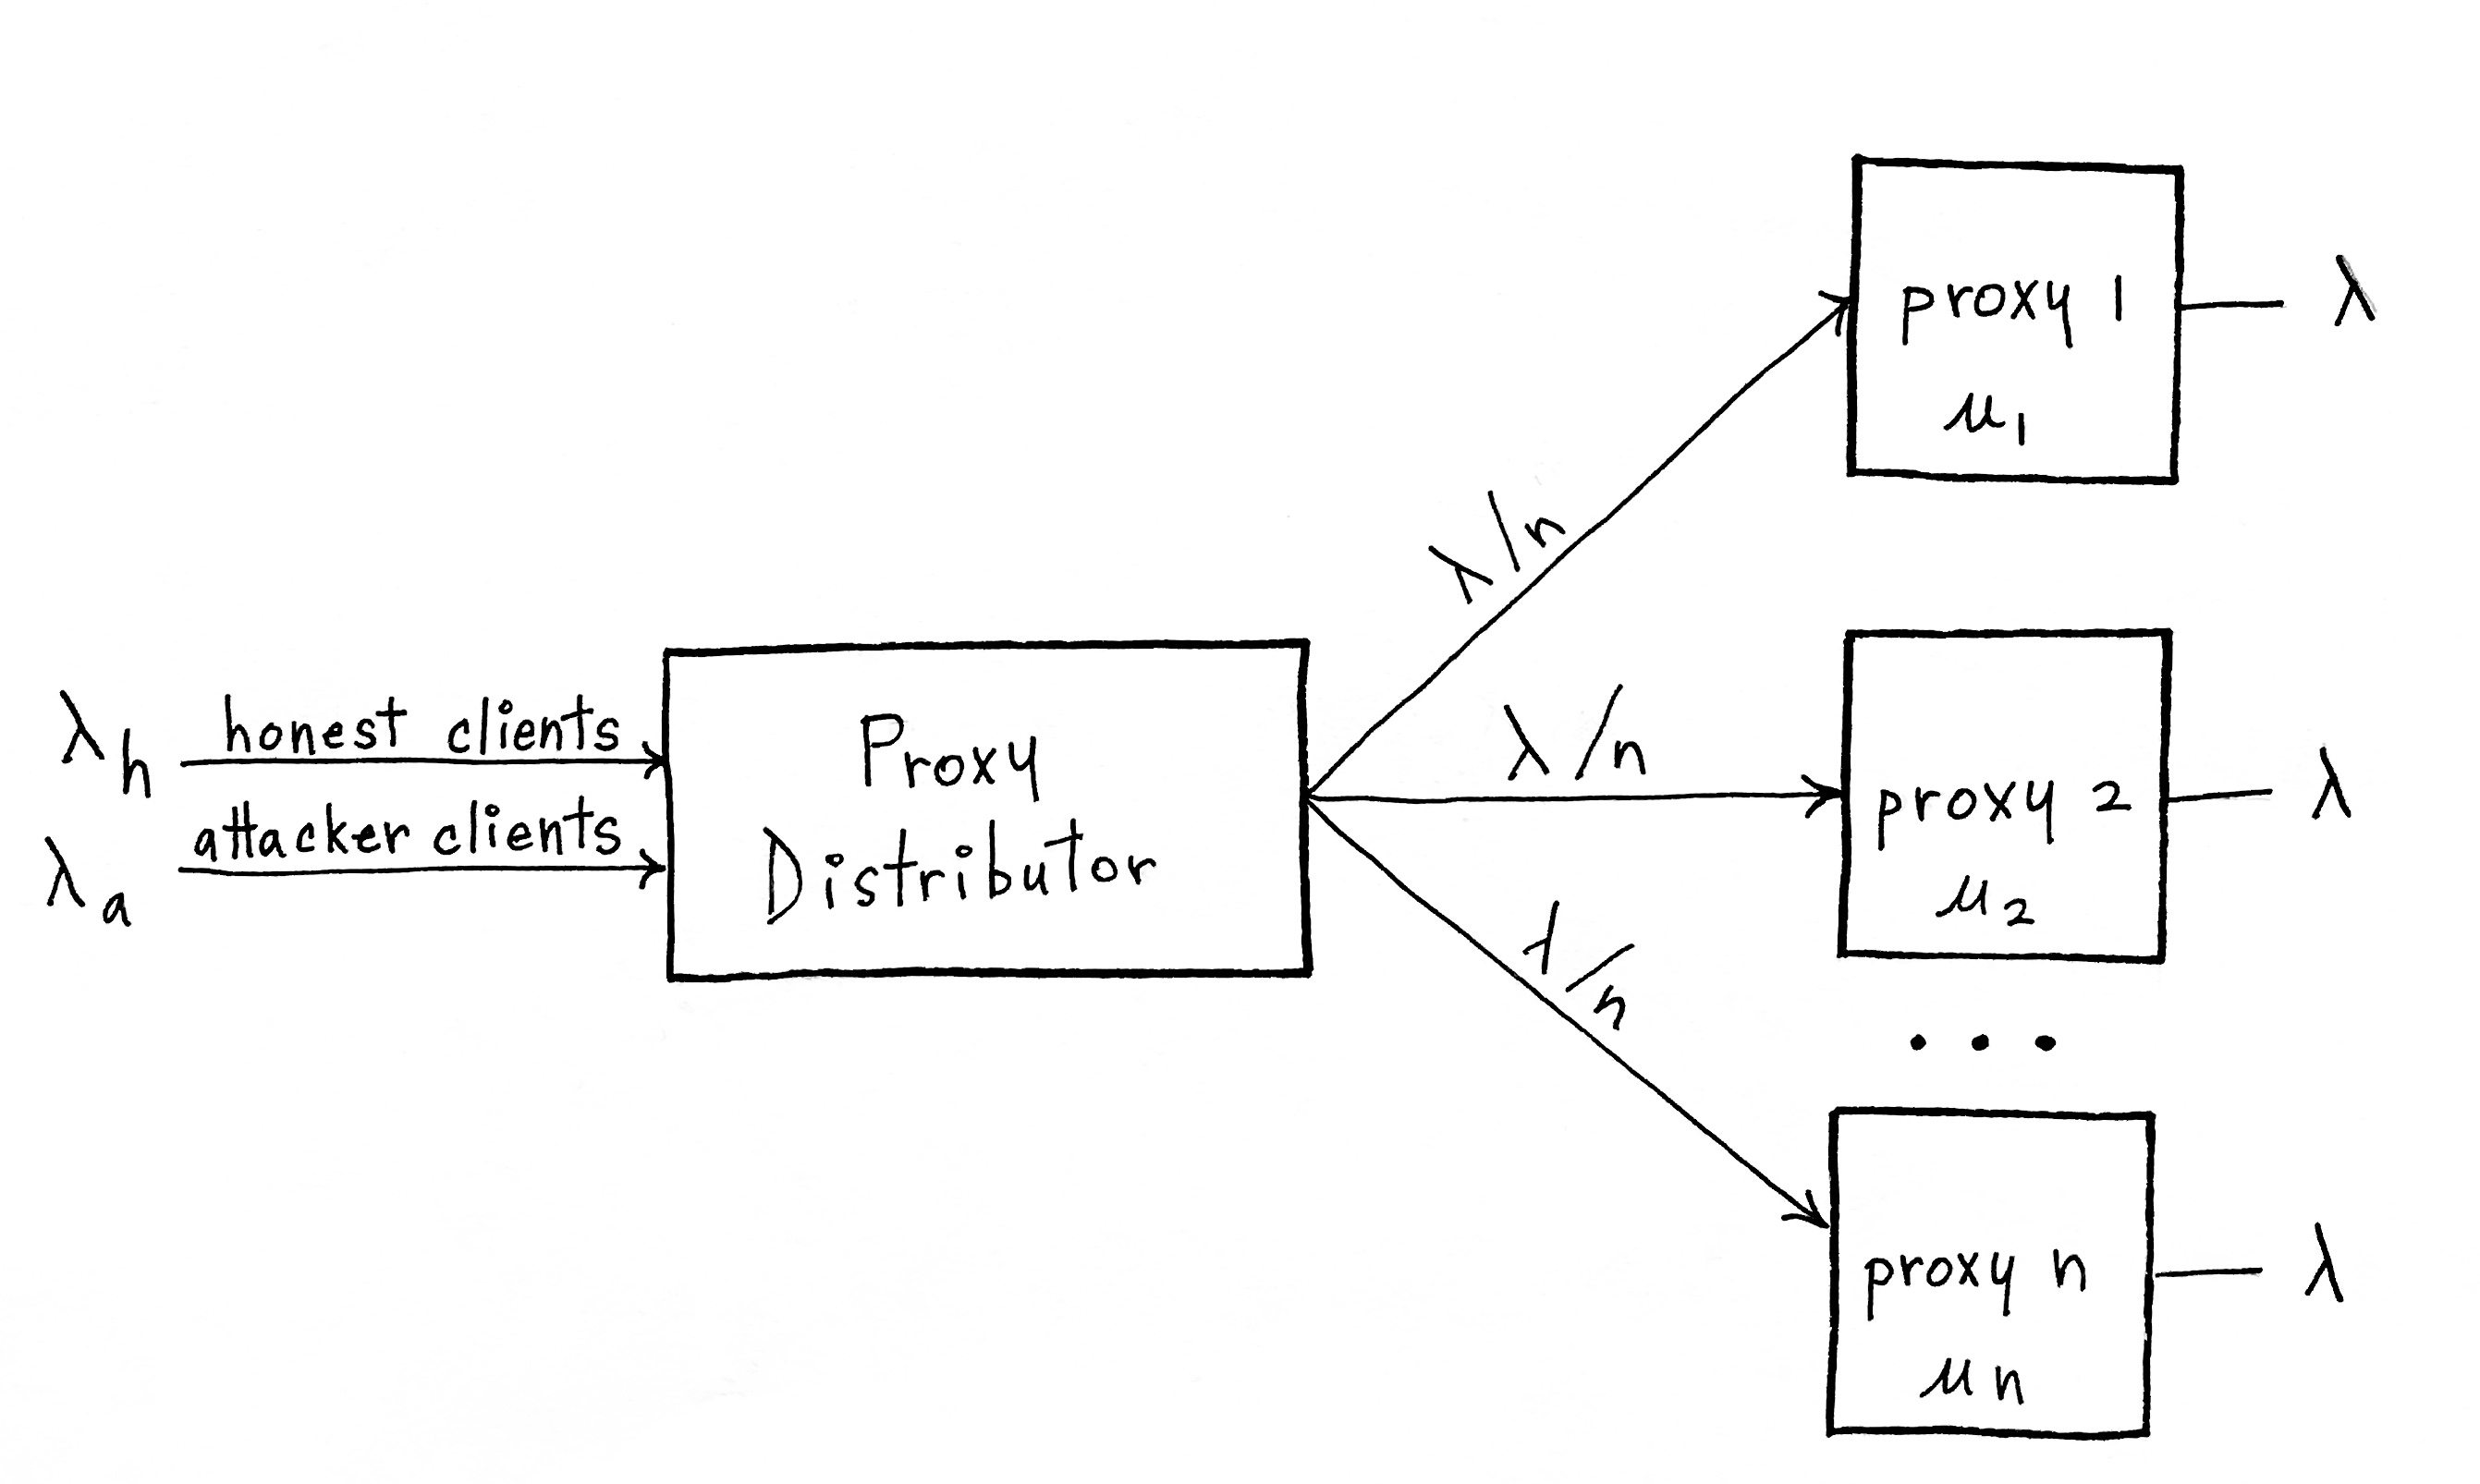
\includegraphics[width=1.0\textwidth]{fig/mmck_queue.png}
    \caption{M/M/c/k with uniform random distribution}

    \label{fig:mmck}
\end{figure*}
%%%%%%%%%%%%%%%%%%%%%%%%%%%%%%%%%%%%%%%%%%%%%%%%%%%%%%%%%%%%%%%%%%%%%%

Clients arrive with a Poisson arrival distribution with variable $\lambda$ clients per minute. This means that, on average, one client appears at every $1 / \lambda$ minutes and we define this as the arrival intensity. In this model, we are additionally concerned with honest and malicious client arrival rates. As the proportion of attackers in the system increases, the arrival rate, or intensity of malicious client arrivals increases.
% TODO define the needle case probability lambda/?, this belongs in the probabilistic analysis above

Each proxy has an service time that is exponentially distributed. This is not a traditional service rate because the system assumes short-lived client connections. The important function of the server is to keep a record of each client assignment that can be used by the censor to discover clients in the system. In other words, even if the client leaves the system, the censor still gains knowledge of the proxy and may affect the client's future connections to the known proxy, effectively mounting a potential future blocking attack on the client, as well as the proxy.

% no longer seems applicable
%We define the aggressive blocking strategy as a censor that blocks each proxy as it is discovered. A complete blocking strategy is a simplified version of delayed blocking where the censor blocks all of the proxies when they are all enumerated, with the assumption that the censor knows the total number of proxies in the system in order to simplify the analysis. The choice of model here is important because it informs the behaviours of an attacker. 

\textbf{Parameters.} Parameters in the simulation control the rate of honest and malicious client arrival intensity, the total number of proxies, and the size of the sliding window for the needle algorithm. These are sweeping parameters; the simulation runs across a range of values for each parameter to produce a variety of conditions for the analysis. The analysis operates on the dependent variables such as maximum load and the expected time to overtake the system. The variable names and descriptions are outlined in the following table:

\begin{table}[h]
  \centering
	\begin{tabular}{ll}
	\hline
	\cline{1-2}
	Parameter Name   & Description  \\
	\hline
    CLIENT ARRIVAL RATE & intensity of client arrival rate \\
	ATTACKER ARRIVAL RATE      & sigma for client arrival rate \\
	NUM PROXIES      & sigma for blocking rate \\
	\hline
	\end{tabular}
  \caption{Variables in the Simulation}
  \label{tab:vars}
\end{table}

The simulator was written in Python using simpy, a discrete event based simulator.\footnote{https://simpy.readthedocs.io/en/latest/} The evaluation uses numpy\footnote{http://www.numpy.org/} and matplotlib\footnote{https://matplotlib.org/} for data manipulation and graphing.

\section{Enumeration Results}

\textbf{Giant step analysis.} We ran the needle algorithm in the simulator, with only malicious attacker clients, to observe how many assignments a censor needs to enumerate all of the proxies. In section \ref{UBGS}, we analyzed the giant step version of the needle algorithm where step size $g > 1$. Asymptotic results are shown in Figure \ref{fig:gsn100} for 1000 trials using 100 proxies in each experiment. The experimental results are shown in the black, solid line. The upper and lower bounds, $E[X] \leq \frac{(n^2)H_{\lceil{H_n}\rceil}}{g}$ and $E[X] \geq (g)(s^2H^{(2)}_{\lfloor{H_n}\rfloor})$ respectively, are shown in dashed lines.

%%%%%%%%%%%%%%%%%%%%%%%%%%%%%%%%%%%%%%%%%%%%%%%%%%%%%%%%%%%%%%%%%%%%%%
\begin{figure*}[h!]
\centering
     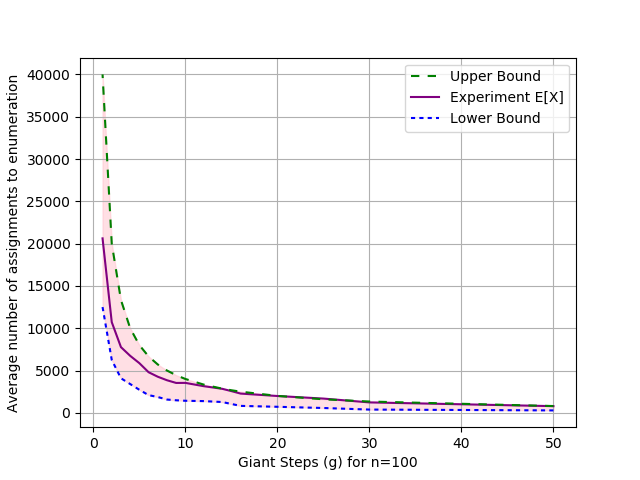
\includegraphics[width=1.0\textwidth]{fig/needle_expected_value_n_100.png}
    \caption{Giant step enumeration comparison for 100 proxies}

    \label{fig:gsn100}
\end{figure*}
%%%%%%%%%%%%%%%%%%%%%%%%%%%%%%%%%%%%%%%%%%%%%%%%%%%%%%%%%%%%%%%%%%%%%%

\textbf{Enumeration Comparison.} We know from the Coupon Collector problem that the uniform random distribution of coupons results in $nH_n$ total assignments before collection. We see that the uniform random distribution of Tor's \texttt{bridgedb} follows a similar enumeration. We use the regular Power of 2 Choices algorithm to show how a more optimal load balancing algorithm results in faster enumeration\cite{xu2011generalized}. In the upcoming section, we'll take a closer look at the load balancing properties of each of these algorithms.

%%%%%%%%%%%%%%%%%%%%%%%%%%%%%%%%%%%%%%%%%%%%%%%%%%%%%%%%%%%%%%%%%%%%%%
\begin{figure*}[h!]
\centering
     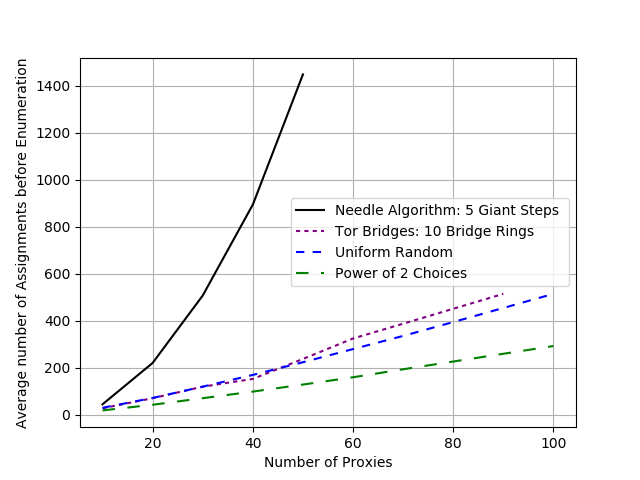
\includegraphics[width=1.0\textwidth]{fig/comparison_graph.png}
    \caption{Enumeration comparison}

    \label{fig:comparison}
\end{figure*}
%%%%%%%%%%%%%%%%%%%%%%%%%%%%%%%%%%%%%%%%%%%%%%%%%%%%%%%%%%%%%%%%%%%%%%

\section{Load Balancing Results}

We observe the needle's load balancing tendencies where the total number of proxies is $n$. Figure \ref{fig:needlelb1} shows the number of proxies sorted by their respective load on the x-axis. The y-axis shows the percentage of the total load that each proxy holds. The maximum load for each of the experiments is no more than 5\% of the total load. This experiment terminates when there are $n$ assignments, so that we can compare our results to known balls-in-bins bounds, shown in Figure \ref{fig:compare1}.

%%%%%%%%%%%%%%%%%%%%%%%%%%%%%%%%%%%%%%%%%%%%%%%%%%%%%%%%%%%%%%%%%%%%%%
\begin{figure*}[h!]
\centering
     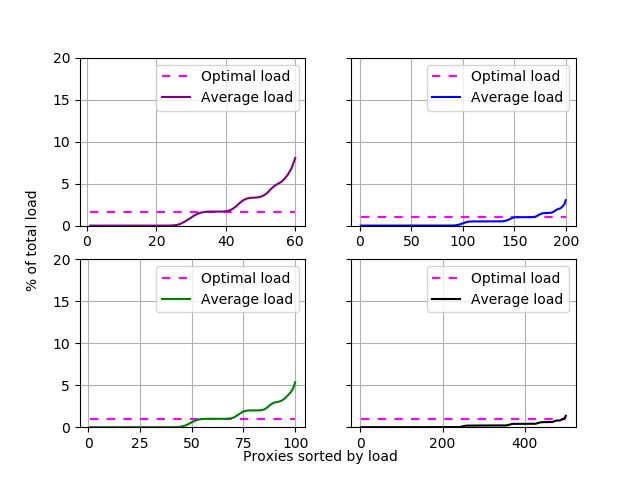
\includegraphics[width=1.0\textwidth]{fig/load_balance_needle_to_n_60_100_200_500.png}
    \caption{Needle Load Balancing where $m=n$ for $n=60, 100, 200, 500$.}

    \label{fig:needlelb1}
\end{figure*}
%%%%%%%%%%%%%%%%%%%%%%%%%%%%%%%%%%%%%%%%%%%%%%%%%%%%%%%%%%%%%%%%%%%%%%


A distinguishing feature of each algorithm is their varying degree of even distribution of assignments to proxies. The power of two choices algorithm gives the most evenly balanced distribution. The uniform random distribution results in the next best load balancing. At the other end of the load balancing spectrum, the $needle$ algorithm results in the worst load balancing.

%%%%%%%%%%%%%%%%%%%%%%%%%%%%%%%%%%%%%%%%%%%%%%%%%%%%%%%%%%%%%%%%%%%%%%
\begin{figure*}[h!]
\centering
     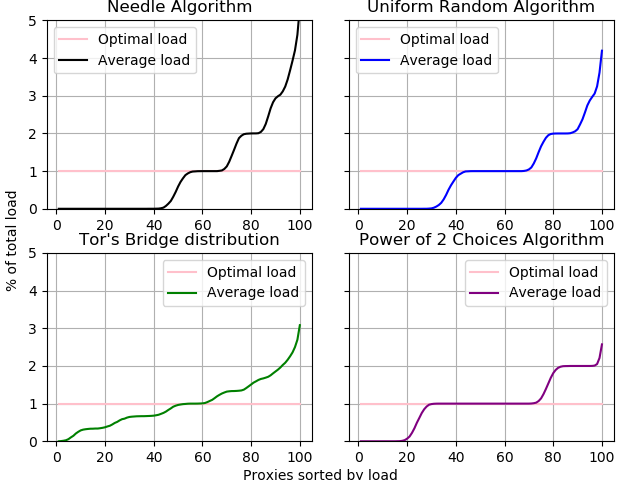
\includegraphics[width=1.0\textwidth]{fig/load_balance_comparison_to_n_100.png}
    \caption{Comparison Load Balancing where $m=n$}

    \label{fig:compare1}
\end{figure*}
%%%%%%%%%%%%%%%%%%%%%%%%%%%%%%%%%%%%%%%%%%%%%%%%%%%%%%%%%%%%%%%%%%%%%%

% TODO what is the maximum load and is it the correct bound loglogn/logn?

%%%%%%%%%%%%%%%%%%%%%%%%%%%%%%%%%%%%%%%%%%%%%%%%%%%%%%%%%%%%%%%%%%%%%%
\begin{figure*}[h!]
\centering
     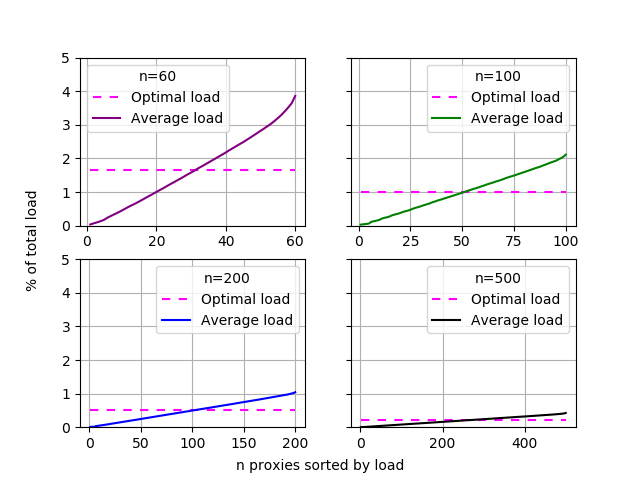
\includegraphics[width=1.0\textwidth]{fig/load_balance_needle_to_twice_enum_60_100_200_500.png}
    \caption{Needle Load Balancing until all proxies are enumerated twice for $n=60, 100, 200, 500$.}

    \label{fig:needlelb2}
\end{figure*}
%%%%%%%%%%%%%%%%%%%%%%%%%%%%%%%%%%%%%%%%%%%%%%%%%%%%%%%%%%%%%%%%%%%%%%


In the experiments shown in Figure \ref{fig:needlelb2}, we ran the needle trials until all of the proxies were enumerated and then kept running the trials until twice the number of enumeration time. Here we see the analysis from Lemma $9$ in section \ref{sec:lb} where $px_{n/2}$ has the optimal load. We see that the load balancing continues to become more divided into two halves centred around the optimal load. 


\section{Bystander Results}

Our bystander results are affected by load balancing and the proportion of attackers in the simulation. For the experiment in Figure \ref{fig:bystandercompare}, we run all of the algorithms so they all have 2000 assignments. We sort the proxies by their loads increasing and show the numbers of malicious attackers assigned to each proxy, from lowest loaded to highest.

%%%%%%%%%%%%%%%%%%%%%%%%%%%%%%%%%%%%%%%%%%%%%%%%%%%%%%%%%%%%%%%%%%%%%%
\begin{figure*}[h!]
\centering
     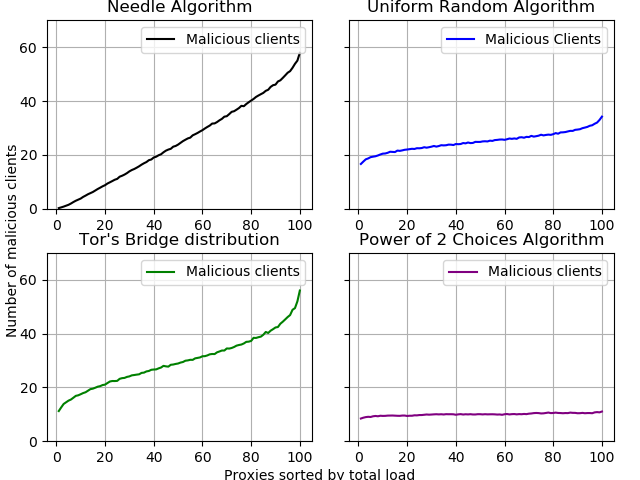
\includegraphics[width=1.0\textwidth]{fig/bystander_comparison_to_n_100.png}
    \caption{Comparison of Malicious Clients}

    \label{fig:bystandercompare}
\end{figure*}
%%%%%%%%%%%%%%%%%%%%%%%%%%%%%%%%%%%%%%%%%%%%%%%%%%%%%%%%%%%%%%%%%%%%%%

We see from the results of this experiment that the number of malicious attackers is increased with load in all of the algorithms, however, in the needle algorithm, lighter loaded proxies have fewer malicious clients. The power of 2 choices algorithm has the flattest distribution of malicious clients, meaning that proxies are enumerated the quickest.

\todo{Graph showing the average total number of bystanders over all experiments (capped at 2000 assignments}


\section{Comparison}

We consider enumeration, load balancing, and bystanders analyses of the four algorithms in order to contrast their respective trade-offs and suitability under differing system goals. Table \ref{tab:tradeoff} outlines the three metrics that we consider in this thesis. We indicate with checkmarks \ding{51} where the algorithm is well suited, double checkmarks indicate that it is very well suited. A single X mark \ding{55} shows that the algorithm is unsuitable, a double \ding{55}  is used when we consider the algorithm to be completely unusable for a purpose.

The Power of 2 Choices algorithm provided the best load balancing, and so would be appropriate for systems where this is a concern. However, it is also enumerated very quickly and has the highest amount of bystanders.

Uniform random distribution and Tor's \texttt{bridgedb} distribution perform similarly, and so we consider their respective trade-offs in the same vein. They provide a slower enumeration time than the Power of 2 Choices algorithm, however, this is due to unevenness in the load balancing. The number of bystanders is not as drastic a drawback as with Power of 2 Choices, but it is not as good as with the Needle algorithm. 

The Needle algorithm gives the slowest enumeration of all the algorithms; this attribute is beneficial to allocation of proxies in a distribution system. It is not suitable for systems that require even load balancing. (It is unbalanced to a large degree but not so much that it is unusable.) Its lower number of bystanders is due to its relatively uneven load balancing. In the context of proxy distribution under our threat model, we consider this a benefit.

\begin{table}[t]
\begin{tabular}{l*{3}{|c}r}
             & Enumeration & Load Balancing & Bystanders \\
\hline
\hline
Power of 2 Choices & \ding{55}\ding{55}  & \ding{51}\ding{51} & \ding{55}\ding{55} \\
Uniform            & \ding{55}  & \ding{51} & \ding{55}  \\
Tor's \texttt{bridgedb} & \ding{55}  & \ding{51} & \ding{55}  \\
Needle           & \ding{51}\ding{51}  & \ding{55}\ding{55}  & \ding{51}\ding{51}  \\
\end{tabular}
\caption{Comparison chart of the 4 algorithms\label{tab:tradeoff} }
\end{table}
%% The following is a directive for TeXShop to indicate the main file
%%!TEX root = diss.tex

\chapter{Related Work} 
\label{sec:related}

%\todo{https://code.briarproject.org/briar/tor-circumvention-analytics/}
%\todo{Enemy at the Gateways}
%\todo{Proxy recycling (unpublished)}

Censorship resistance systems \ac{CRS} are composed of two parts; 1) communication establishment, or handshake, needed to join the \ac{CRS}, and 2) the conversation stage where the actual information is exchanged between the client and the censored site. In \textit{SOK: Making sense of censorship resistance systems} \cite{khattak2016sok}, categorizations of different types of \ac{CRS} are outlined based on the system's approach to these two functions. 

There are two main approaches to communication establishment in censorship resistance systems; resource scheduling and allocation approach, and the trust-based approach. Resource scheduling and allocation fight a losing battle to distribute proxies under a censorship threat model where proxies are continuously blocked. Proxies need to be birthed or placed into reserve in order to keep up with the censor's blocking rate. The advantage of these schemes is that they are lightweight and easy to implement.

The goal of trust-based proxy distribution is to mitigate blocking by building trust between honest users of the system and the proxy distributor. They achieve this by distinguishing honest clients from malicious clients. We outline systems and techniques that fall under a similar censorship threat model as our own, where the censor is omnipotent and blocks proxies based on information gained by posing as an honest user.

Note that other types of anonymous systems, such as Vuvuzela \cite{vandenHooff:2015:VSP:2815400.2815417}, Dissent \cite{corrigan2010dissent}, and Freenet \cite{clarke2001freenet}, are concerned with maintaining levels of anonymity in order to prevent an adversary from learning about messages from a sender to a receiver. The highest level of anonymity in these systems is a \textit{third axis} where one cannot tell that a user is communicating with any other user \cite{reiter1999anonymous}. The adversary in the proxy distribution problem under a censorship threat model is vastly stronger than in general anonymity systems. The goal of \ac{CRS} is to obfuscate evidence that a user is in the system at all, as well as the activity of the user within said system.

\section{Resource Scheduling and Allocation}

\textbf{Tor's Bridge Distribution.} Tor bridges are private relays or proxies used for censorship circumvention. Tor bridge \ac{IP} addresses and fingerprints are distributed out of band using registered email or through a captcha site on the Tor blog. Tor's BridgeDB authority distributes up to 3 new bridge IPs and corresponding fingerprints to clients based on a hashring uniform distribution. Bridge requests are rate limited by a centralized bridge distributor. Despite these efforts, censors in China have discovered and blocked most of the bridges given through the public distribution channels. Bridge enumeration attacks are possible using bulk emails via \ac{HTTPS} \cite{ling2015tor}. Tor uses a fingerprint as a shared secret scheme to thwart active probing, however this can't prevent bridge discovery using a delayed insider attack \cite{fifield2016censors}. \\

\textbf{TorBricks.} The TorBricks \cite{zamani2017torbricks} design distributes proxies in groups to guarantee a maximum number of rounds until all honest users can connect to a proxy server after some number of retries. It relies on exponential growth in the number of proxies in order to provide these guarantees of a logarithmic number of rounds. A caveat in this system is, if there are no unblocked proxies in the current group, then the algorithm requires that a unique bridge be allocated per each user. 

While this approach allows for adaptive adjustment to a proportion of attackers in the system, it requires a great deal of resources. For example, if a \ac{CRS} had enough proxies to give one out per each user, we would not have the problem of proxy distribution since we could hand out private proxies. If we have private proxies, then no attacker could discover an honest user's proxy because users would not have to share.\\

\textbf{Fighting Censorship with Algorithms.}
Mahdian \cite{mahdian2010fighting} studies proxy distribution as an algorithmic problem and gives bounds on the number of proxies required to provide service to clients, some of whom are adversaries. He includes a theoretical analysis of bounds for the number of proxies needed to survive an insider attack. His theorems use k-union-free families of sets, probabilistic methods, and extremal set theory to give lower and upper bounds. 

Mahdian's scheme creates two sets of users, trusted and suspicious, and distributes keys based on the user's membership in one of these two sets. Users are divided into these sets based on their association with compromised keys; they are moved from the trusted group to the suspicious group. Fresh keys are only handed out to trusted users. This adaptive model bounds the number of keys that an adversary can compromise thus providing guarantees for the user with respect to the expected total number of keys required to give every legitimate user access.

In Mahdian's model, a key represents a servlet or proxy server. His scheme assumes a known number of malicious users and there are no bounds on the number of clients a proxy can serve. While maintenance of keys is usually relatively simple in practice, the logistics of proxy server maintenance is more involved. It is an impractical assumption that keys (representing proxies) can be distributed to an unlimited number of users without significant overhead. 

Mahdian's algorithm distributes an increasing number of keys to users in order to reduce the risk posed by a growing number of adversaries. This does not address the case where adversaries are controlled by the same entity, such as a censor. For example, it does not take into consideration the enumeration attack. This attack is further exacerbated by the reuse of keys, as opposed to the removal of suspect keys.\\


\section{Trust-based Allocation}

%\todo{HYPHAE: Social Secret Sharing https://patternsinthevoid.net/hyphae/hyphae.pdf}

\textbf{Proximax.} The main goal of the Proximax \cite{mccoy2011proximax} reputation-based system is to maximize the yield of a proxy resource, where yield is the number of user-hours per day before a proxy is blocked, calculated as the product of usage and lifetime. Each proxy resource is advertised on multiple channels. This novel use of a channel relies on a fast flux technique that piggybacks on \ac{DNS} infrastructure. Proximax registers multiple proxies to the same domain name and load balances them based on their current utilization and resource risk parameter. 

The usage and risk of a proxy resource is the sum of the risk of each of the channels where it is distributed. Resource risk is calculated as a maximum likelihood estimate of blocking - it is only an approximation because resources are advertised on multiple channels, and the risk per channel cannot be sampled directly. In other words, when a proxy is blocked, there is no way to detect the specific channel that caused the block and so it is difficult to tease out channel from proxy risk. 

All proxies will eventually be discovered in proxy distribution, so Proximax adds a trust scheme to delay censor discovery. Registered users build up their reputation score and invite new users, handled by a registration system. The registration system allocates proxies that have higher risk to lower reputation scores. They widely disseminate the location of low risk proxies in order to maximize their yield. This leads to the potential of rapid enumeration attacks, where the best proxies are enumerated in quick succession. 

Proximax's trust scheme is likely to be thwarted by colluding insider attackers where registered users build up reputation to invite other users, as it does not work well in a delayed blocking attack. Furthermore, the risk approximation may not be particularly useful because if there is only a single attacker assigned to a proxy, and with the reasonable assumption that all attackers are controlled by the same censor entity, then this proxy has the same likelihood of being blocked as a proxy to which several insider attackers are assigned. \\

\textbf{rBridge.} rBridge \cite{wang2013rbridge} is a trust-based reputation system for a Tor bridge distributor that addresses insider attacks, minimizes user wait time for an available proxy, and preserves privacy of client assignment information. The rBridge distributor computes user reputation based on the uptime of bridges to which a user is assigned. A payment system allows users to buy unblocked bridges to prevent repeated blocks. They show rBridge's user-hours served is at least one order of magnitude more than Proximax and that thirsty hours of users waiting for a proxy is minimized. This is mainly achieved by making sure that the overall rate of new bridges outpaces the rate of proxy blocks, and by reserving half of their bridge resources for future invitations.

A significant contribution of rBridge's design is their privacy preserving scheme using anonymous credentials to build trust, invite users, and obtain signed credentials. Restricting proxy assignments can lead to user fingerprinting as there are unique combinations of proxies tied to a single user. Previous work in pseudonymous credentials and oblivious transfer methods don't work well in proxy systems because an attacker can still infer client assignments based on behaviour after a proxy is blocked. rBridge hides bridge assignment from even the distributor by enabling the proxy assignments to be written and updated by users. They take extra measures to maintain integrity using anonymous credentials, one-time tokens and secrets that cannot be forged owing to zero knowledge proofs and blind signatures. 

In addressing the delayed blocking attack, they note that invitation tickets are randomly distributed over all users, so there is a chance that the corrupt user may not receive a ticket. Since tickets cannot be transferred, it is no more likely that an attacker receives a ticket than an honest user. However, they do not provide analysis given that even just one corrupt user is more than enough to block a proxy, therefore an assignment of a proxy to a single attacker is more significant than assignment to an honest user. \\


\section{Routing}

Routing users through decoy paths as a mechanism to discover proxies is a vastly different approach to the proxy distribution problem and handshake used in censorship resistance systems. Essentially, this approach solves the issue of censors posing as honest users and blocking proxies because censors do not want to block the decoy paths. This is because there would be too much collateral damage as the decoy paths are heavily used and it is difficult to tell if users are accessing blocked sites from the decoys. The barrier to implement these solutions, however, is that they require a large commitment from either \ac{CDN} or \ac{ISP} to build the decoy paths and to maintain the network that provides the anonymous handshake.\\

\textbf{Telex.} This \ac{CRS} uses destination obfuscation via decoy routing at Telex stations that are \textit{end-to-middle} proxies located in their own network infrastructure \cite{wustrow2011telex}. Sessions between users and Telex have special tags to direct them through to censored sites. These proxies are built into the network with involvement from local \ac{ISP} that must deploy Telex stations on paths between networks under censor control and blocked destinations.\\

\textbf{Domain Fronting.} An elegant way to circumvent censors is through domain fronting, where a user is routed through a legitimate intermediary, such as a \ac{CDN} \cite{Fifield2017a}. These intermediaries are used to rendezvous with Tor and cannot be detected by a censor because the \ac{CDN}'s network is beyond the censor boundary. Domain fronting is the most reliable way to perform the rendezvous handshake and recently it is the only protocol that works in China \cite{TORDOMAIN:2019}. However, we see that major \ac{CDN} like Google and Amazon no longer support domain fronting. Microsoft's Azure cloud is a temporary fix as there is no formal agreement between Microsoft and Tor to support domain fronting in the future.\\

\section{Related Approaches}

The following works aren't directly related to the problem of censorship circumvention. However, their analysis of resource allocation is closely tied to the coupon collector analysis in this thesis. Their lightweight distribution under a different threat model also relates to and inspired our approach.\\

\textbf{Coupon Collector and Power of d Choices.} The Power of d Choices was analyzed for the generalized form of the coupon collector problem in \cite{xu2011generalized}. This includes the case where a collector wants to collect $m$ out of $n$ total coupons. The collector selects $d$ coupons out of the total collection and chooses the least heavily loaded (or least collected) coupon in each draw. This benefits the collector because duplicate coupons are discarded. They show that the expected number of draws to collect $m$ out of a total of $n$ coupons is $(n \log{n})/d + (n/d )(m − 1) \log{\log{n}} + O (mn)$. Although this is opposite from our reverse power of 2 choice algorithm, and far more complex in its analyses, it is a useful counterpoint to our goal of delaying enumeration, as the goal here is to enable the coupon collector to collect coupons as quickly as possible.\\

\textbf{Proxisch.} Proxisch \cite{jiang2016proxisch} is an application of a scheduling algorithm for proxy distribution in web crawling applications. Although Proxisch is intended for distributed web crawling, the proxy server selection mechanism has a similar goal shared by the proxy distribution problem; to reduce the risk of assigning high risk proxies to clients. This work estimates the reliability of proxies based on a reliability calculation and uses queuing theory to organize proxies by their respective reliability factors. 

To model the life of a proxy, they use an exponential distribution based on the life of an ideal lamp. They show in their simulations that the actual life span of some proxy servers is close to the exponential distribution. This leads to the calculation of an optimal update period for cycling proxies among processes. They compare their result to a polling scheduling solution that illustrates higher successful service rates within shorter time periods for their solution. Their resource scheduling algorithm approach is similar to a randomized proxy selection based on attributes of proxies, such as time, reputation, or credits because it orders proxies based on criterion. This is a move away from more complex, monolithic designs favouring proxies that earn standing over time within the system. 

It's not possible to directly translate this solution into the problem addressed in this thesis, since modeling the lifetime of a proxy server does not directly translate to the motivations of a powerful censor that can cut the lifetime of a proxy at any time. However, this work does provide useful hints for how one may approach a lightweight proxy distribution design.\\



\chapter{Discussion}
\label{sec:discussion}

\section{Future Work}

\textbf{Blocking behaviour.} The simulation can easily extend to model different forms of blocking behaviour by a censor. The parameters for a blocking rate process are coded in the simulation although these were not utilized in the simulation nor analyzed for the evaluation.  

\textbf{Proxies joining and leaving.} A more realistic version of the simulator is to run the experiments with some proxies joining and leaving. This would provide more data on how the needle algorithm preserves new proxies, rather than only dealing with proxies that are created at the same time.

\textbf{Service times.} The simulation was not fully utilized to analyze classic problems like Quality of Service. It would be particularly interesting to examine how non-needle proxies are able to handle the larger loads in a real system.

\textbf{Tor integration.} The needle algorithm could be run inside of the Tor bridedb codebase to validate the simplicity of the algorithm's approach. It would require a different method of client assignment because Tor uses hashes of IP addresses and does not store load or assignment information in the same way that the needle algorithm requires for its operation.
\chapter{Conclusion}
\label{sec:conclusion}

My work has the same goal as many trusted proxy distribution systems outlined in the related work in Chapter \ref{sec:related}; to provide service to clients in a hostile environment with practically an omnipotent censor entity. This trust-less, elegant approach to proxy distribution relies on essentially hiding \textit{needle} proxies in distribution rounds.

Building trust requires storage of user statistics over time. Within anonymous systems, the assumption that any user can be trusted to build reputation is an extremely complex topic, both technically and ideologically. While it can be argued that seemingly all proxies provide a measure of anonymity because multiple users are aggregated on a single proxy, there exists a fundamental distrust of any proxy distribution system that persists user information, as it goes against the ethos of anonymity. 

%    2. Main body
% Generally recommended to put each chapter into a separate file
%\include{relatedwork}
%\include{model}
%\include{impl}
%\chapter{Discussion}
\label{sec:discussion}

\section{Future Work}

\textbf{Blocking behaviour.} The simulation can easily extend to model different forms of blocking behaviour by a censor. The parameters for a blocking rate process are coded in the simulation although these were not utilized in the simulation nor analyzed for the evaluation.  

\textbf{Proxies joining and leaving.} A more realistic version of the simulator is to run the experiments with some proxies joining and leaving. This would provide more data on how the needle algorithm preserves new proxies, rather than only dealing with proxies that are created at the same time.

\textbf{Service times.} The simulation was not fully utilized to analyze classic problems like Quality of Service. It would be particularly interesting to examine how non-needle proxies are able to handle the larger loads in a real system.

\textbf{Tor integration.} The needle algorithm could be run inside of the Tor bridedb codebase to validate the simplicity of the algorithm's approach. It would require a different method of client assignment because Tor uses hashes of IP addresses and does not store load or assignment information in the same way that the needle algorithm requires for its operation.
%\include{conclusions}

%    3. Notes
%    4. Footnotes

%    5. Bibliography
\begin{singlespace}
\raggedright
\bibliographystyle{abbrvnat}
\bibliography{biblio}
\end{singlespace}

\appendix
%    6. Appendices (including copies of all required UBC Research
%       Ethics Board's Certificates of Approval)
%\include{reb-coa}	% pdfpages is useful here
%\section*{Appendix A}


\backmatter
%    7. Index
% See the makeindex package: the following page provides a quick overview
% <http://www.image.ufl.edu/help/latex/latex_indexes.shtml>


\end{document}
